\documentclass[a4paper,12pt]{scrreprt}
\usepackage[ngerman]{babel}
\usepackage[left=2cm,right=2cm,top=2.5cm,bottom=2.5cm]{geometry}
\usepackage{amsmath}
\usepackage{acronym}
\usepackage{amsfonts}
\usepackage{amssymb}
\usepackage{makeidx}
\usepackage{graphicx}
\usepackage{epstopdf}
\usepackage{kpfonts}
\usepackage[utf8]{inputenc}
\usepackage[T1]{fontenc}
\usepackage{textcomp}
\usepackage[onehalfspacing]{setspace}
\usepackage[colorlinks=true, allcolors=blue]{hyperref}
\usepackage[backend=biber,style=apa]{biblatex}
\addbibresource{references.bib}
\newcommand{\dcplace}{Aachen}
\newcommand{\dcdate}{04. Mai 2025}
\newcommand{\dcauthorfirstname}{Max}
\newcommand{\dcauthorlastname}{Mustermann}

\usepackage{fancyhdr}
\pagestyle{fancy}
\fancyhf{}
\fancyhead[L]{\nouppercase{\leftmark}} % Kapitelname in normaler Schrift
\fancyhead[R]{} 
\setlength{\parindent}{0pt}
\fancyfoot[C]{\thepage} 

\usepackage{listings}
\usepackage{xcolor}
\definecolor{bggray}{gray}{0.95}
\definecolor{codeblue}{rgb}{0.1, 0.1, 0.8}
\definecolor{codered}{rgb}{0.8, 0.1, 0.1}
\definecolor{codegreen}{rgb}{0.1, 0.6, 0.1}
\definecolor{codeorange}{rgb}{0.9, 0.5, 0.1}
\lstset{
	basicstyle=\ttfamily\small\color{codeblue},
	backgroundcolor=\color{bggray},
	keywordstyle=\color{codered}\bfseries,
	stringstyle=\color{codegreen}, 
	commentstyle=\color{gray}\itshape, 
	breaklines=true, 
	showspaces=false,
	showstringspaces=false,
	showtabs=false,
	tabsize=2
}
\lstdefinelanguage{properties}{
	morecomment=[l]{\#},
	morecomment=[s]{/*}{*/},
	morestring=[b]",
	basicstyle=\ttfamily\small\color{codeblue},
	keywordstyle=\color{codeorange}\bfseries,
	commentstyle=\color{codegreen}\itshape,
	backgroundcolor=\color{bggray},
	breaklines=true,
	showspaces=false,
	showstringspaces=false,
	showtabs=false,
	tabsize=2
}
\lstdefinelanguage{POM}{
	language=XML,
	basicstyle=\ttfamily\small\color{codeblue},
	keywordstyle=\color{codeorange}\bfseries,
	stringstyle=\color{codegreen},
	backgroundcolor=\color{bggray},
	morekeywords={dependency, groupId, artifactId, version, dependencies},
	breaklines=true,
	showspaces=false,
	showstringspaces=false,
	showtabs=false,
	tabsize=2
}

\definecolor{dkgreen}{rgb}{0,0.6,0}
\definecolor{gray}{rgb}{0.5,0.5,0.5}
\definecolor{mauve}{rgb}{0.58,0,0.82}

\lstset{
	language=Java,
	aboveskip=3mm,
	belowskip=3mm,
	showstringspaces=false,
	columns=flexible,
	basicstyle={\small\ttfamily},
	numbers=none,
	numberstyle=\tiny\color{gray},
	keywordstyle=\color{blue},
	commentstyle=\color{dkgreen},
	stringstyle=\color{mauve},
	breaklines=true,
	breakatwhitespace=true,
	tabsize=3,
	inputencoding=utf8,
	literate={ä}{{\"a}}1 {ö}{{\"o}}1 {ü}{{\"u}}1 {Ä}{{\"A}}1 {Ö}{{\"O}}1 {Ü}{{\"U}}1 {ß}{{\ss}}1
}

\usepackage{float}

\begin{document}
	\begin{titlepage}
		%ab hier kleinere Raender, mehr bedruckbare Flaeche.
		\thispagestyle{empty}
		\newgeometry{a4paper, portrait, left=1.0cm, right=0cm, top=0.6cm, bottom=0cm, includefoot}
		
		\noindent
		\begin{minipage}[t]{0.5\textwidth}
			
\includegraphics[width=3.7cm]{firmenlogo.jpg}
		\end{minipage}%
		\begin{minipage}[t]{0.5\textwidth}
			\raggedleft
			
\includegraphics[width=1.7cm]{FHAC.jpg}
		\end{minipage}
		
		\vspace{1.0cm}
		
		% Kopfzeile mit Fachbereich ...
		{\centering \bfseries \Large FH~Aachen \\
			\vspace{1cm}
			\normalsize Fachbereich\\
			Elektrotechnik und Informationstechnik \\
			Studiengang~Informatik \par}
		
		\vspace{1cm}
		
		{\centering \bfseries \large Bachelorarbeit \par}
		
		\vspace{1cm}
		
		\centering \begin{minipage}[t]{13cm}
			\centering \small Konzeption und prototypische Entwicklung einer webbasierten Applikation zur Wertschöpfung und Bereitstellung von Geodaten \\
			(Data-Konnector für Geodaten)
			\medskip
		\end{minipage}
		
		\vspace{1.5cm}
		
		%\vspace*{1cm}
		%\hspace*{6.8cm}
		\begin{minipage}[t]{9cm}
			\centering Tuan Anh Cong Nguyen \\ Matr.-Nr.: 3517392
		\end{minipage}
		\vspace{2.1cm}
		
		%\vspace*{4.7cm}
		%\hspace*{6.8cm}
		\centering \begin{minipage}[b]{15cm}
			\centering
			Referent: Prof. Dr. rer. nat. Heinrich Faßbender\\
			%Korreferent: Prof. Dr.-Ing. ...\
		\end{minipage}
		
		
		\vspace{1.5cm}
		
		%Erstellungsdatum
		%\vspace{-4cm}
		%\begin{flushright}
		\centering %\hspace{8cm}
		\begin{minipage}[b]{10cm}
			\centering
			In Zusammenarbeit mit Ausbildungsbetrieb:\\
			ahu GmbH Wasser Boden Geomatik \\
			\vspace{1cm}
			Externer Betreuer: Dr. David Loibl
			
			%\today\\ %Datum\\
			%\vspace{1cm}
			%vertraulich bis xx.xx.xx
		\end{minipage}
		%\end{flushright}
		
		%\today
		\restoregeometry
	\end{titlepage}
	
	\clearpage % Neue Seite für Selbstständigkeitserklärung
	\chapter*{Selbstständigkeitserklärung}
	\thispagestyle{empty}	%keine Seitenzahl!
	\pdfbookmark{Selbstständigkeitserklärung}{Selbstständigkeitserklärung}
	Ich versichere hiermit, dass ich die vorliegende Arbeit selbständig verfasst und keine anderen als die im Literaturverzeichnis angegebenen Quellen benutzt habe.\\ \\
	Stellen, die wörtlich oder sinngemäß aus veröffentlichten oder noch nicht veröffentlichten Quellen entnommen sind, sind als solche kenntlich gemacht.\\ \\ Die Zeichnungen oder Abbildungen in dieser Arbeit sind von mir selbst erstellt worden oder mit einem entsprechenden Quellennachweis versehen.\\ \\ Diese Arbeit ist in gleicher oder ähnlicher Form noch bei keiner anderen Prüfungsbehörde eingereicht worden.\\ \\[2ex]
	Aachen, den \today \hspace{4cm} \dotfill 
	\tableofcontents
	
	\clearpage
	\chapter*{Abkürzungsverzeichnis}\label{abkuerzungsverzeichnis}
	\begin{acronym}[\hspace{3cm}]
		\acro{REST-API}{Representational State Transfer Application Program Interface}
		\acro{OGC}{Open Geospatial Consortium}
		\acro{WMS}{Web Map Server}
		\acro{WFS}{Web Feature Server}
		\acro{JSON}{JavaScript Object Notation}
		\acro{CSV}{Comma Separated Values}
		\acro{ASCII}{American Standard Code for Information Interchange}
		\acro{QGIS}{Quantum Geographic Information System}
		\acro{UI}{User Interface}
		\acro{HTML}{Hypertext Markup Language}
		\acro{CSS}{Cascading Style Sheets}
		\acro{HTTP}{Hypertext Transfer Protocol}
		\acro{URL}{Uniform Resource Locator}
		\acro{AJAX}{Asynchronous JavaScript and XML}
		\acro{J2EE}{Java 2 Platform, Enterprise Edition}
		\acro{XML}{Extensible Markup Language}
		\acro{JAR}{Java Archive}
		\acro{WAR}{Web Application Archive}
		\acro{JPA}{Java Persistence API}
		\acro{CRUD}{Create, Raed, Update and Delete}
		\acro{UUID}{Universally Unique Identifier}
		\acro{SRP}{Single Responsibility Principle}
	\end{acronym}
	
	\cleardoublepage
	\chapter*{Abstract}
	\thispagestyle{plain}
	\addcontentsline{toc}{chapter}{Abstract}
	In einer zunehmend digitalisierten und automatisierten Welt wächst täglich die Menge an neu generierten Geodaten – insbesondere Mess- und räumlichen Daten.\\ \\
	Die Suche nach und Einbindung von OGC-Geodatendiensten wie WMS (Web Map Service) und WFS (Web Feature Service) in Geoinformationssysteme wie QGIS kann tatsächlich schwierig sein. Die Suche erfordert den Anwender oft das Durchforsten verschiedener Quellen und die manuelle Überprüfung von Dienstbeschreibung. Eine automatisiert und effiziente Lösung kann teilweise helfen, diesen Prozess zu verbessern. \\ 
	Die Suche nach Messdaten wie Grundwasserständen, Pegelständen und Klimadaten (Niederschlag,Temperatur) und deren Umformatierung in ein einheitliches Format gestalten sich als schwierig und kompliziert, da es eine Vielzahl von Datenanbietern mit unterschiedliche Datenstrukturen, Formen, etc. gibt.\\ \\
	Die Bereitstellung dieser Rohdaten erfolgt meinst im CSV-Format oder als individuell strukturierte ASCII-Dateien. Im Kontext von der Datenkonsum, gibt es bei der Ahu den sogenannten ahuManager-Client, der diese Daten konsumiert. Bevor diese konsumieren können, müssen die Rohdaten in ein kompatibles Format umformatiert werden, was bisher teilweise von Hand erledigt werden (in Excel o.ä.). Diese manuelle Vorgehen kann perspektivisch zum Teil oder ganz automatisiert werden, was die Produktivität steigert und die Fehleranfälligkeit vermeidet. \\ \\
	Daher befasst sich diese Arbeit  mit dem Thema, wie eine webbasierte Applikation zur Wertschöpfung und Bereitstellung von rohen Geodaten im Kontext von der Abteilung Geomatik von Ahu GmbH entwickelt werden kann.
	
	\clearpage
	\chapter{Einleitung}
	\section{Motivation der Arbeit}
	Diese Bachelorarbeit wird in Zusammenarbeit mit dem Bereich Geomatik der Ahu GmbH verfasst.Der Bereich beschäftigt sich mit Konzeption und Softwareentwicklung der Monitoringsysteme und Web-Anwendungen, die es Dienstleitern, Betreibern und Aufsichtsbehörden ermöglichen, ein kosteneffizientes Management für Geodaten(Grundwasser, Oberflächenwasser, Boden,etc.) umzusetzen. \\ \\
	Momentan besteht es Bedarf für ein zentrales System zur automatisierten Suche und Verwaltung der Geodaten aus verschiedenen Datenanbietern und diese Daten in einer homogen Struktur zusammenzubringen und einen vorhandenen Client(z.B ahuManager) bereitzustellen. Unter anderem  wird auch die Einbindung von OGC-Geodatendiensten für besseren und effizienten Prozess zur Durchsuche und Verwaltung gesorgt. 
	
	\section{Ziel der Arbeit}
	Die Hauptaufgabe dieser Arbeit besteht darin, ein Konzeption für die prototypische Entwicklung einer webbasierten Applikation zu erstellen und umzusetzen. Die Ziele enthalten eine übergreifende Suche von Geodaten und deren Umformatierung in ein passendes vorgegebenes Zielformat. Das weitere Zeil ist die Einbindung von mindestens einer OGC-Geodatendiensten.\\ \\ Durch die Umsetzungen dieser Ziele soll perspektivisch eine Software entstehen, die offene Problematik eine mögliche Lösung anbietet.
	
	\section{Aufbau der Arbeit}
	\section*{\small \textbf{Kapitel 1: Einleitung}}
	Im ersten Kapitel werden die Motivation und Zwecke für diese Arbeit erklärt. Es wird kurz auf die Problematik des gewählten Themas eingegangen und dieses perspektivisch für die Firma auch Vorteile bringt.
	
	\section*{\small \textbf{Kapitel 2: Übersicht von Technologien}}
	In diesem Kapitel werden wichtige Begriffe und in der Entwicklungsphase verwendete Technologien vorgestellt. Von der Bibliothek zur Verfolgung der Datenbankänderungen über das Backend-Framework bis hin zu in der Benutzeroberfläche verwendetem UI-Framework.   
	\section*{\small \textbf{Kapitel 3: Anforderungsanalyse und Spezifikation}}
	In diesem Kapitel werden verschiedene User-Stories definiert und daraus Use-Cases spezifiziert, was die funktionale und nicht-funktionale Anforderungen der Anwendung angeht.  
	\section*{\small \textbf{Kapitel 4: Konzeption und Architektur}}
	Dieses Kapitel erläutert die Entscheidung für die gewählte Architektur des Prototyps anhand von unterschiedlichen Sichten.
	\section*{\small \textbf{Kapitel 5: Implementierung}}
	Anhand zahlreichen Code-Beispiele und technischen Erläuterungen wird die wirkliche Implementierung nochmal veranschaulicht. 
	\section*{\small \textbf{Kapitel 6: Evaluierung}}
	Das vorletzte Kapitel bewertet, inwiefern die vom Anfang festgelegte und erarbeitete Anforderungen erfüllt wurde. 
	\section*{\small \textbf{Kapitel 7: Fazit und Ausblick für weitere Entwicklung}}
	Abschließend wird noch einmal die gesamte Arbeit zusammenfassend bewertet und ein kurzer Ausblick für weiteren Entwicklungen oder Verbesserungen in der Zukunft gegeben.
	
	\chapter{Übersicht von Technologien}
	\section{Vaadin}
	Vaadin ist ein serverseitiges Web-Framework, das dem Entwickler erlaubt, moderne Webanwendung in Java zu entwickeln, ohne dass explizit HTML,CSS oder JavaScript geschrieben werden muss. Vaddin verfügt über eine große Komponentenbibliothek, die eine Vielzahl an vorgefertigten UI-Elementen wie Buttons, Tabellen, Formulare, Dialoge und Layouts bietet.
	
	\begin{figure}[h!]
		\centering
		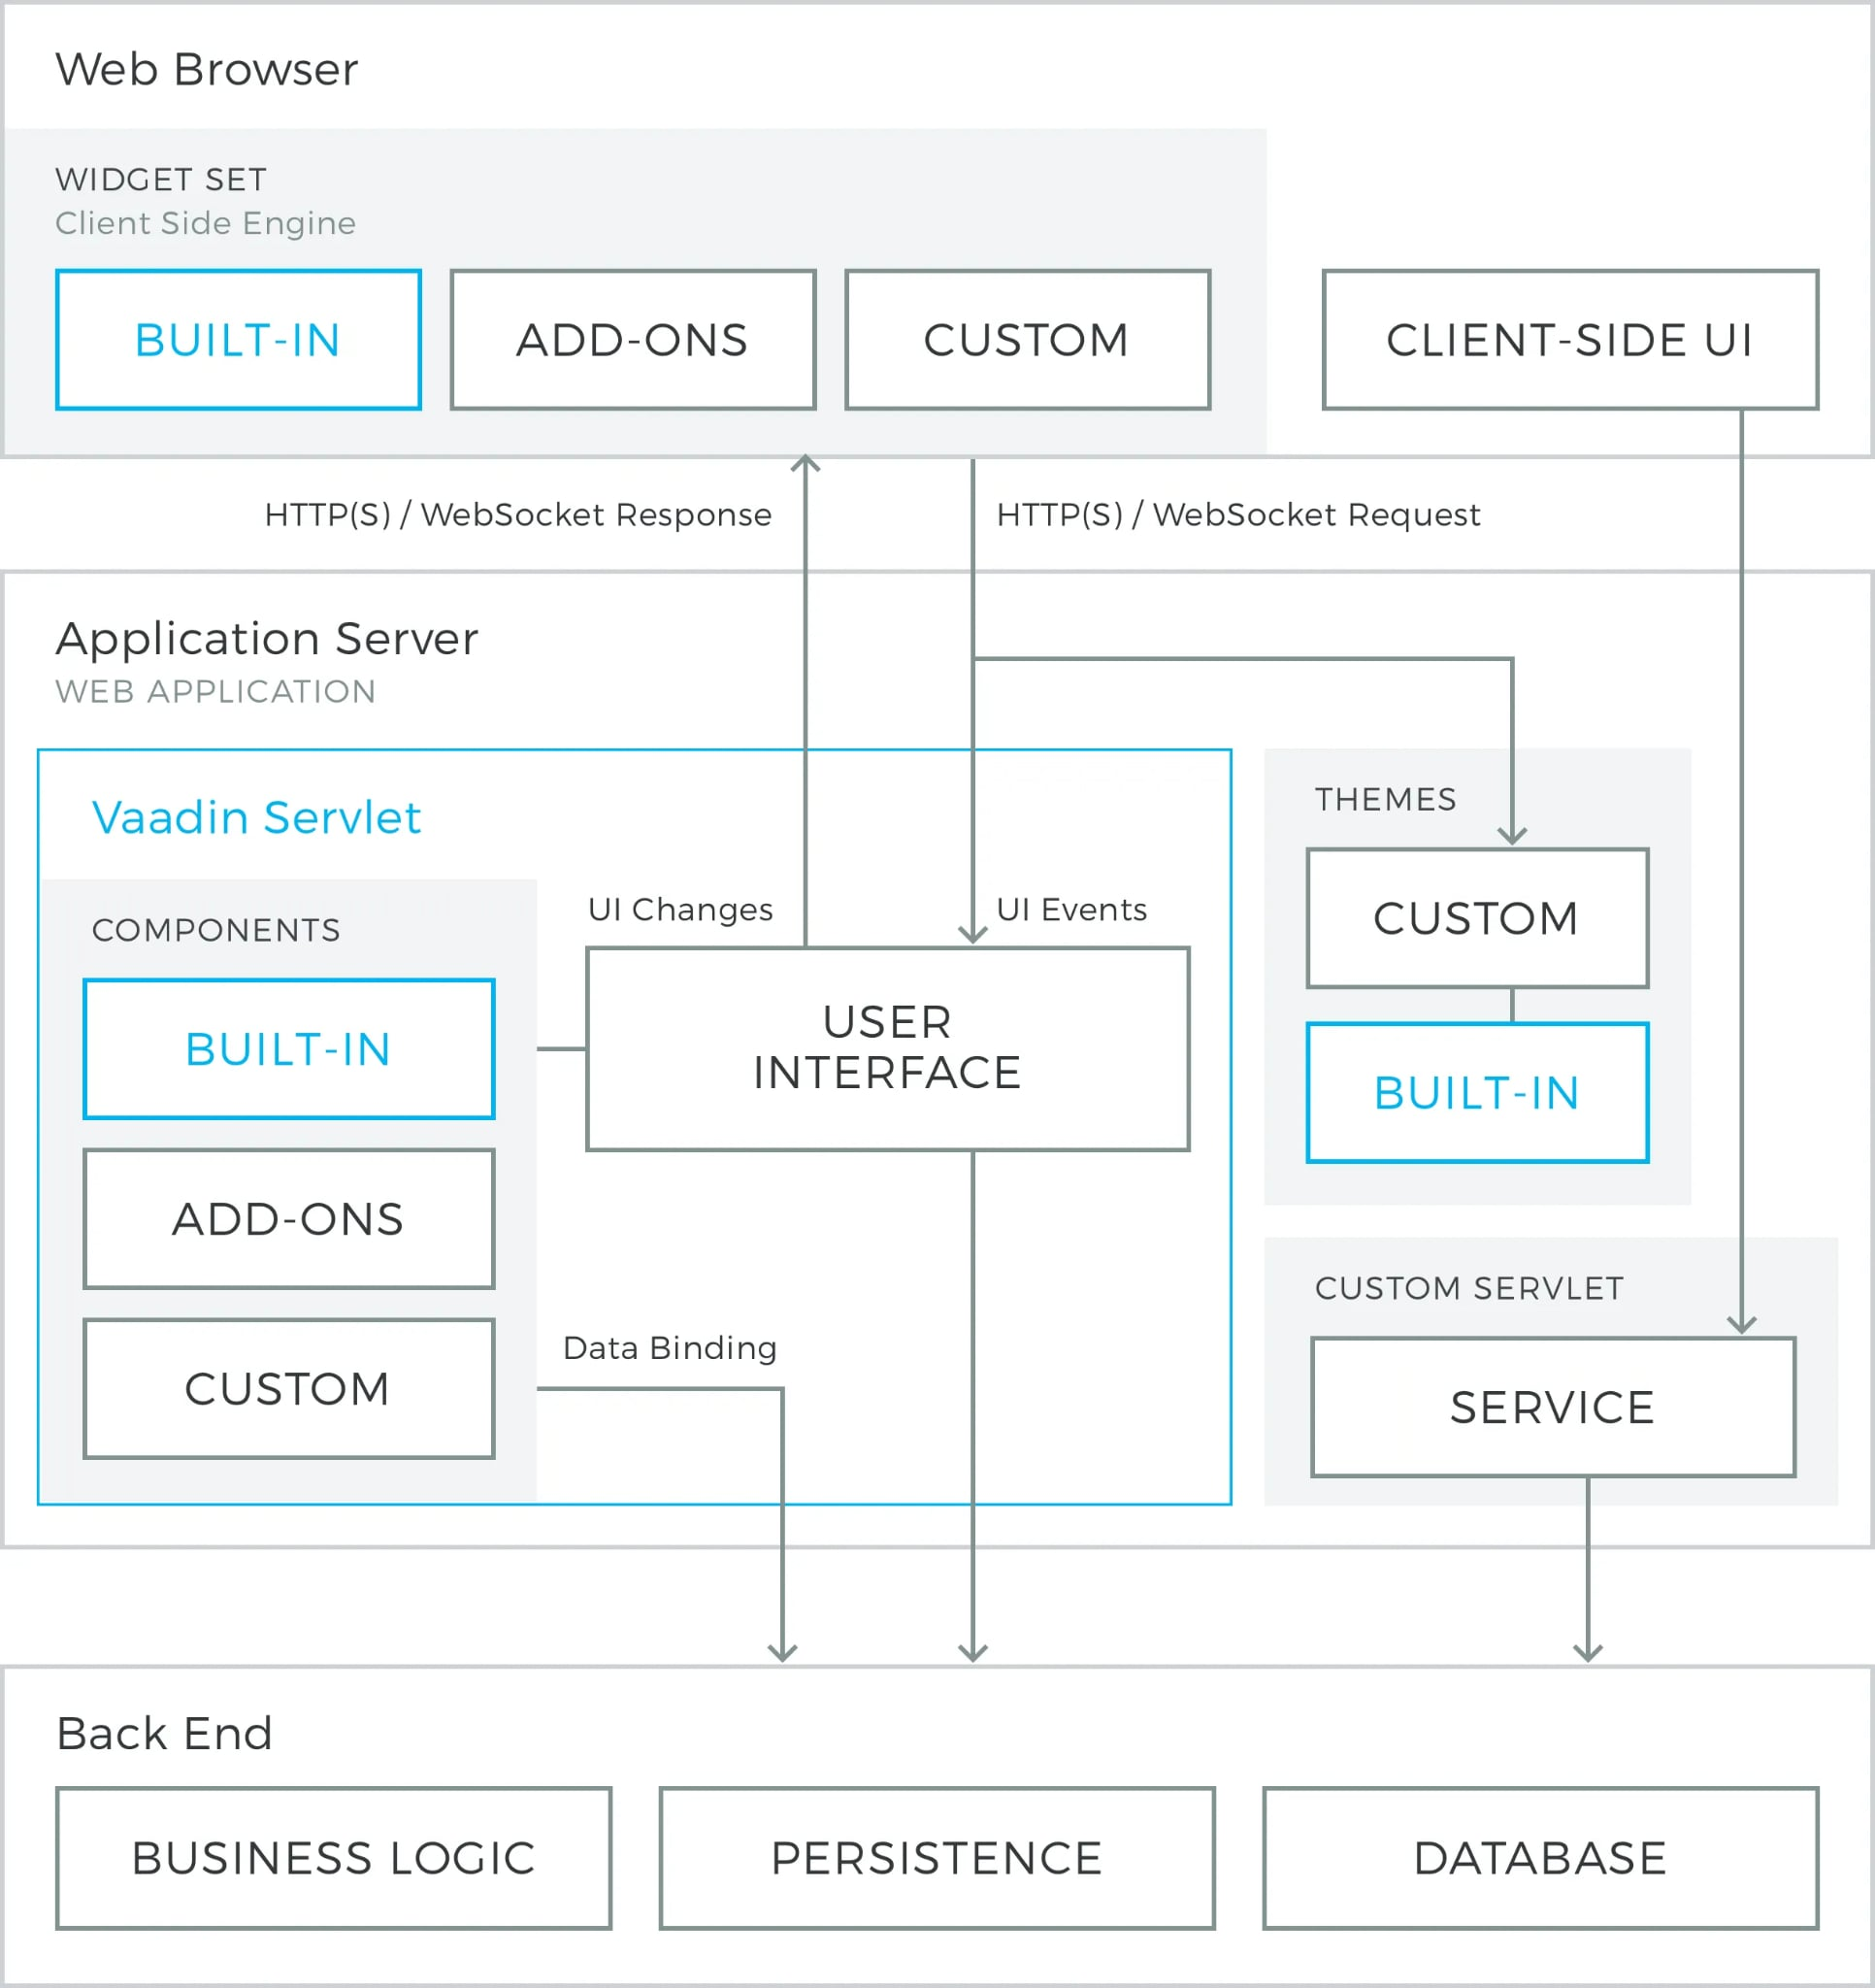
\includegraphics[width=9cm, height=10cm]{vaadin_architekture.jpg}
		\caption{\label{vaadin:architektur}Übersicht Vaadin Architektur \cite{architecture21}}
	\end{figure}
	Vaadin verfolgt einen serverseitigen Rendering-Ansatz. Während eine AJAX-basierte Vaadin Client-Side Engine dafür sorgt, dass die Benutzeroberfläche im Browser durch ein Widget-Set gerendert wird. Die Benutzeroberfläche kann aus eingebauten Komponenten, Add-Ons und benutzerdefinierten Komponenten bestehen. Diese Client-Side Engine kommuniziert über HTTP oder WebSockets mit dem Server. Die gesamte UI-Logik wird dann auf dem Server ausgeführt. Die Vaadin Servlet empfängt Client-Anfragen und aktualisiert die Benutzeroberfläche. Die UI-Komponenten werden serverseitig erstellt und verwaltet. Änderungen in der UI werden durch die Vaddin Client-Side Engine an den Browser zurückgespielt.  
	
	\section{Spring Framework}
	Spring Framework ist ein Java-Framework, das um 2003 als Reaktion auf die damals noch zu komplizierte J2EE-Plattform entwickelt wurde. Spring ermöglicht eine einfachere und unkompliziertere Entwicklung von Enterprise-Applikation in Java. Eines der wichtigsten Konzepte von Spring war die Inversion of Control (IoC).
	IoC ist ein Prinzip, bei dem der Kontrollfluss an eine externe Quelle(z.B. ein Framework) übergeben wird. Das Framework ist dann gemäß einer Spezifikation für die Erstellung und Löschung der Objekte und den Aufruf von Methoden verantwortlich. \\ \\ Spring führt das Konzept des Bean-Containers ein. Beans sind Java-Objekte, die von Spring instanziiert und verwaltet sind. Wenn die Haupt-Bean von der Hilfs-Bean abhängig ist, stellt Spring sicher, dass die Hilfs-Bean vor der Haupt-Bean initialisiert wird. Spring injizierte außerdem die Instanz der Hilfs-Bean in die Haupt-Bean, sodass die Haupt-Bean nicht mehr nach ihren eigenen Abhängigkeiten suchen muss. Dieses Muster wird als Dependendy Injection bezeichnet.\\ \\
	Damals musste der Entwickler die Bean-Konfiguration in XML schreiben, die Spring anweist, wie die Beans zu konstruieren sind. Inzwischen wird diese mithilfe einer Kombination aus Java-Annotation, Java-Code und Konventionen erstellt.
	\section{Spring Boot}
	Mit dem Wachstum der Spring-Plattform nahm auch die Komplexität der Entwicklung von Spring-Anwendungen zu. Gleichzeitig verbreitet sich der Einsatz von Microservices und containerisierten Umgebungen in der Softwareentwicklung. Entwickler wünschten sich einfach Methode, um schlanke Webanwendungen zu erstellen, die unabhängig als eigenständige Dienst ausgeführt werden können, anstatt auf einem dedizierten Anwendungsserver zu laufen.\\ \\
	Spring Boot wurde als Reaktion auf diese Anforderungen entwickelt. Es erleichtert die Erstellung von Spring-Anwendungen durch sinnvolle Standard-Einstellungen, Starter-Abhängigkeiten und produktionsreife Funktionen für Konfiguration und Überwachung. Durch die Einführung eingebetteter Servlet-Container wurde es möglich, Anwendungen als eigenständige, ausführbare JAR-Dateien zu verpacken. 
	\section{Maven}
	Maven ist ein Build-Management- und Projektverwaltungswerkzeug, das häufig in der Java-Entwicklung eingesetzt wird. Es automatisiert Aufgaben wie das Herunterladen von Abhängigkeiten, das Kompilieren von Quellcode und das Ausführen von Builds sowie Tests. Maven verwendet eine zentrale Konfigurationsdatei, die \texttt{pom.xml}, um alle Aspekte des Projekts wie Libraries, Plugins und Build-Prozesse zu steuern.\\ \\
	Die Funktionsweise von Maven basiert auf einem deklarativen Ansatz. Das bedeutet, dass der Entwickler alle relevanten Informationen über das Projekt in einer zentralen Konfigurationsdatei, der sogenannten \texttt{pom.xml}( Projekt Object Model) angibt, wie z.B. Abhängigkeiten, Build-Prozesse und Plugins : \cite{deinhard24}.
	\section*{\small \textbf{1. Die pom.xml-Datei (Project Object Model)}}
	Die \texttt{pom.xml} ist das Herzstück eines Maven-Projekts. Sie enthält Informationen wie:
	\begin{itemize}
		\item Projektinformationen: Name des Projekts, Version, Beschreibung.
		\item Abhängigkeiten: Welche Bibliotheken und Framworks das Projekt benötigt.
		\item Plugins: Zusätzliche Werkzeuge, die den Build-Prozess erweitern (z.B. Compiler-Plugins, Test-Frameworks).
		\item Repositories: Woher Maven externe Abhängigkeiten herunterladen soll, typischerweise das Maven Central Repository.
		\item Build-Spezifikationen: Kompilierungsanweisungen, Testkonfigurationen und Deployment-Optionen.
	\end{itemize}
	\section*{\small \textbf{2. Build-Lifecycle}}
	Maven besitzt einen vordefinierten Build-Lifecycle, der aus mehreren Phasen besteht. Zu den wichtigsten Phasen gehören:
	\begin{itemize}
		\item validate: Überprüft, ob alle erforderlichen Informationen im Projekt vorhanden sind.
		\item compile: Kompiliert den Quellcode.
		\item Führt automatisierte Tests aus.
		\item package: Verpackt den kompilierten Code in ein Distributionsformat, typischerweise eine JAR- oder WAR-Datei.
		\item install: Installiert das Paket in das lokale Maven-Repository, damit es in anderen Projekten verwendet werden kann.
	\end{itemize}
	
	\section{Vaadin Initializer}
	Gegenüber dem üblichen \href{https://start.spring.io/} {Spring Initializer}, der ein vorkonfiguriertes Spring-Projekt bereitstellt, bietet der \href{https://start.vaadin.com/app/p} {Vaadin Initializer} den Vorteil, dass er speziell auf Vaadin-Projekte zugeschnitten ist und eine vereinfachte und schnellere Projektgenerierung ermöglicht, insbesondere wenn man Spring Boot als Backend verwendet.\\ \\ Mit dem Vaadin- Initializer kann man direkt ein Vaadin Flow-basiertes Projekt mit einem Spring Boot-Backend erstellen, während man mit dem Spring Initializer ein allgemeines Spring Boot-Projekt generiert und dann manuell die Vaadin-Abhängigkeiten hinzufügen muss.
	
	\section{Liquibase}
	Dank Versionsverwaltung wie Git kann man in den meisten Projekten den Weg einer Code-Änderung von der der Entwicklung über Test bis hin zum produktiven Deployment richtig verfolgen und nachvollziehen. Was für den Code gilt, sollte auch für die Datenbankanpassungen gelten. Liquibase ist eine Bibliothek um Änderungen an einem Datenbankschema verfolgen, verwalten und anwenden zu können. Mit folgendem Eintrag in \texttt{pom.xml} kann man in ein Spring-Projekt integrieren.
	\begin{lstlisting}[language=POM]
		<dependency>
		<groupId>org.liquibase</groupId>
		<artifactId>liquibase-core</artifactId>
		<version>4.23.1</version>
		</dependency>
	\end{lstlisting}
	Für die Speicherung der Daten wird die PostgreSQL-Datenbank entschieden. PostgreSQL selbst eine leistungsstarke, offene Datenbank, die kompatibel zu Liquibase passt. Die Aktivierung der Datenbank wird in der Datei \texttt{application.properties} innerhalb der Spring-Applikation wie folgt konfiguriert:
	\begin{lstlisting}[language=properties]
		spring.datasource.url=jdbc:postgresql://192.168.252.140:5432/opendataconn_ng
		spring.datasource.driver-class-name=org.postgresql.Driver
		spring.datasource.username=opendataconn_ng_usr
		spring.datasource.password=
		spring.jpa.database-platform=org.hibernate.dialect.PostgreSQLDialect
		spring.liquibase.change-log=classpath:/db/changelog-root.xml
	\end{lstlisting}
	Für die Verwendung von Liquibase sind folgende Dateien notwendig:
	\begin{figure}[h!]
		\centering
		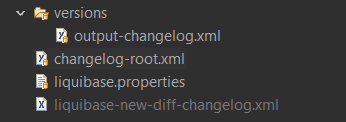
\includegraphics[width=9cm, height=3cm]{liquibase-changelog.png}
		\caption{\label{datenbank:konfiguration} Liquibase-Konfiguration}
	\end{figure}
	\section*{\small \textbf{1. Liquibase Konfiguration - liquibase.properties}}
	In dieser Datei werden allgemeine Einstellungen wie der Datenbankzugang und die zu verwendenden Changelog-Konfiguration festgelegt.
	\begin{lstlisting}[language=properties]
		# Database Configuration
		url=jdbc:postgresql://192.168.252.140:5432/opendataconn_ng
		username=opendataconn_ng_usr
		password=
		driver=org.postgresql.Driver
		# Reference Configuration
		referenceUrl=hibernate:spring:de.ahu.opendata?dialect=org.hibernate.dialect.PostgreSQLDialect
		referenceDriver=liquibase.ext.hibernate.database.connection.HibernateDriver
		# Output Files
		changeLogFile=src/main/resources/db/changelog-root.xml
		diffChangeLogFile=src/main/resources/db/liquibase-new-diff-changelog.xml
		outputChangeLogFile=src/main/resources/db/versions/output-changelog.xml
	\end{lstlisting}
	\section*{\small \textbf{2. Changelog Konfiguration - changelog-root.xml}}
	Ein so genannter Root-ChangeLog wird erstellt, welcher in XML geschrieben ist und eine output-changelog.xml inkludiert, welche im Ordner ,,versions'' zu finden ist. Diese Datei sorgt dafür, dass Liquibase das ChangeSet findet.
	\begin{lstlisting}
		<?xml version="1.0" encoding="UTF-8"?>   
		<databaseChangeLog
		xmlns="http://www.liquibase.org/xml/ns/dbchangelog"
		xmlns:xsi="http://www.w3.org/2001/XMLSchema-instance"
		xmlns:pro="http://www.liquibase.org/xml/ns/pro"
		xsi:schemaLocation="http://www.liquibase.org/xml/ns/dbchangelog
		http://www.liquibase.org/xml/ns/dbchangelog/dbchangelog-4.23.xsd
		http://www.liquibase.org/xml/ns/pro 
		http://www.liquibase.org/xml/ns/pro/liquibase-pro-4.23.xsd">  
		<includeAll path="db/versions"/>  
		</databaseChangeLog>
	\end{lstlisting}
	\section*{\small \textbf{3. Changelog Konfiguration - output-changelog.xml}}
	Diese Datei enthält sämtliche Datenbankänderungen und die Änderungen werden in Form von ChangeSet beschrieben und verwaltet.Im Folgenden ist ein Abschnitt im XML-Format für das Anlagen einer Tabelle Abonnement wiedergegeben. \\ 
	\begin{lstlisting}
		<changeSet author="ng (generated)" id="1743435452264-1">
		<createTable tableName="abonnement">
		<column name="id" type="VARCHAR(32)">
		<constraints nullable="false" primaryKey="true" primaryKeyName="abonnementPK" />
		</column>
		<column name="description" type="TEXT" />
		<column name="label" type="VARCHAR(255)">
		<constraints nullable="false" />
		</column>
		<column name="base_url" type="VARCHAR(255)" />
		<column name="file_format" type="VARCHAR(255)" />
		<column name="end_datum" type="date" />
		<column name="location_id" type="VARCHAR(255)" />
		<column name="parameter" type="VARCHAR(255)" />
		<column name="start_datum" type="date" />
		<column name="sub_url" type="VARCHAR(255)" />
		</createTable>
		</changeSet>
	\end{lstlisting}
	\section*{\small \textbf{4. Changelog Konfiguration - liquibase-new-diff-changelog.xml}}
	Diese Datei enthält nur bestimmte Änderungen von bestimmten Tabellen, die man in die Datei \texttt{output-changelog.xml} einfügt, wenn man das Schema der Datenbank modifiziert. Ähnlich wie in \texttt{output-changelog.xml} werden Änderungen auch in Form von ChangeSet beschrieben.
	
	\section{Datenbankmanagementsystem}
	Wie bereits in dem letzten Abschnitt offengelegt, wird ein PostgreSQL als das Datenbankmanagementsystem gewählt. 
	Da alle Datenbanken von Ahu GmbH zentral im lokalen Netzwerk liegen und die meisten Projekte PostgreSQL-Datenbank verwenden, ist es deswegen ersichtlich, dass für dieses Projekt auch eine PostgreSQL-Datenbank verwendet wird. \\
	Außerdem spricht der Einsatz einer PostgreSQL-Datenbank aufgrund ihrer zahlreichen Vorteile für sich.
	\begin{enumerate}
		\item Open-Source: geringe Kosten und hohe Flexibilität und Innovation, die bei anderen Datenbanklösung nicht immer möglich sind. 
		\item Leistung und Skalierbarkeit : PostgreSQL unterstützt eine Vielzahl von Leistungsoptimierung und verfügt über eine hohe Lese-/Schreibgeschwindigkeit, insbesondere bei der Unterstützung von Geodaten.
		\item Fundierte Sprachunterstützung : Aufgrund seiner Kompatibilität und Unterstützung mehrerer Programmiersprachen ist PostgreSQL eine der flexibelsten Datenbanken für Entwickler. Python, JavaScript, C/C++, Java und weitere beliebte Programmiersprachen bieten ausgereifte Unterstützung für PostgreSQL.
	\end{enumerate}
	
	\chapter{Anforderungsanalyse und Spezifikation }
	\section{Analyse}
	Während der Analysephase werden die \textbf{\textit{Stakeholder}} identifiziert und deren Anforderungen mittels \textbf{\textit{User Stories}} gesammelt. Die Anforderungen können in drei verschiedenen Untergruppen eingeteilt werden, um die systematisch und spezifisch behandeln zu können.
	\begin{enumerate}
		\item Funktionale Anforderungen beschreiben die Funktionen, die eine ganze Anwendung oder auch nur eine von ihren Komponenten erfüllen soll. Eine Funktion besteht aus drei Schritten: Eingabe der Daten-Systemverhalten-Ausgabe der Daten. Sie kann die Daten berechnen und manipulieren, Geschäftsprozesse ausführen, Benutzerinteraktionen herstellen oder andere Aufgabe ausführen.
		\item Nicht-funktionale Anforderungen beschreiben, wie das System es tut, während die funktionalen Anforderungen bestimmen, was das System tut. Darunter zählen die Leistungsstandards und Qualitätsmerkmale von Software, z.B. die Benutzerfreundlichkeit, Effektivität, Sicherheit, Skalierbarkeit usw.
		\item Randbedingungen sind Vorgaben, die den Lösungsraum einschränken und das Verhalten der Software beeinflussen.
	\end{enumerate}
	\subsection{Anwendungsszenario}
	Die zu entwickelnde Applikation soll als zentrale Stelle für die Durchsuche der Geodaten und Verwaltung der relevanten Geodaten dienen und ist auch in der Lage, diese Geodaten durch eine Schnittstelle einen anderen Client zur Verfügung stellen zu können.
	\subsection{Stakeholder}
	In der Softwareentwicklung sind Stakeholder Personen, Gruppen oder Organisation, die ein Interesse am Erfolg eines Softwareprojekts haben und von dessen Ergebnissen direkt oder indirekt beeinflusst werden.
	
	\subsection{User-Stories}
	Mittels User-Stories können funktionale Anforderungen der Stakeholder erfasst werden.
	\begin{enumerate}
		\item Als Benutzer möchte ich in der Web-Oberfläche eine Übersicht über populäre Datenquellen sehen, die  relevante Geodaten bereitstellen.
		\item Als Benutzer möchte ich mithilfe von Schlagwörtern nach OGC-Webservices durchsuchen und die entsprechenden Referenzen als URL-Links zu den Schlagwörtern erhalten.
		\item Als Benutzer möchte ich gezielt nach Messdaten wie Grundwasserständen, Pegelständen, Niederschlag, etc. recherchieren und dabei Informationen über das Datenformat und wesentliche Inhalte der Datensätze erhalten.
		\item Als Benutzer möchte ich Messdaten, die meist im CSV-Format oder individuell strukturierte ASCII-Dateien vorliegen, in ein passendes Zielformat konvertieren lassen.
		\item Als Benutzer möchte ich die Daten in Form einer List von Datenstreams angezeigt bekommen.
		\item Als Benutzer möchte ich in der Lage sein, bestimmte Datensätze abonnieren zu können.
		\item Als Benutzer möchte ich die gefundenen Geo- und Messdaten visuell auf einer Karte darstellen lassen.
	\end{enumerate}
	
	\section{Spezifikation}
	Mit den im letzten Abschnitt erhobenen User-Stories können nun die funktionalen Anforderung genauer spezifiziert werden. Dort werden Use-Cases genauer definiert.
	\subsection{Use-Cases}
	Einfach ausgedrückt wird mit einem Use-Case die nach außen sichtbare Interaktion eines Nutzers mit einem System dokumentiert. Dieser Nutzer kann entweder eine Person, eine Organisation oder ein anderes System sein.\\
	Für die prototypische Anwendung werden folgenden Use-Cases ausgearbeitet.
	\section*{\small \textbf{Use-Case 1: Historische Wetterdaten von \href{https://wetterdienst.readthedocs.io/en/latest/} {Wetterdatendienst} einsehen}}
	Akteur : Benutzer\\
	Ziel: Historische Wetterdaten einer bestimmten Messtation einsehen\\
	Vorbedingung: keine\\
	Nachbedingung: keine\\
	\underline{Ablauf}:
	\begin{enumerate}
		\item Benutzer navigiert zu Historische Wetterdaten Tab.
		\item Am Anfang zeigt die Seite einige Dropdowns zur Durchsuche der Daten und eine Karte, auf der noch keine Station zu sehen ist.
		\item Benutzer wählt die gewünschte Auflösung aus (stündlich, täglich, monatlich, jährlich).
		\item Benutzer wählt dann die Hauptparameter aus und ein Dropdown für Unterparamter blendet sich ein.
		\item Benutzer wählt anschließend die Unterparamter aus.
		\item Das System reagiert auf den Wert von Unterparamter und zeigt sich eine deutschlandweite Karte, wo alle relevanten Messstationen zu dem ausgewählten Unterparamter zu sehen sind. 
		\item Weitere Dropdowns werden danach eingeblendet, entweder möchte Benutzer die Messstationen in einem bestimmten Bundesland sehen oder direkt eine gezielte Messstation auswählen.
		\item Nach Auswahl einer Station wird die Station auf der Karte fokussiert und die Daten zur gewählten Station als Diagramm dargestellt. 
	\end{enumerate}
	\section*{\small \textbf{Use-Case 2: Wettervorhersagedaten von \href{https://wetterdienst.readthedocs.io/en/latest/} {Wetterdatendienst} einsehen}}
	Akteur : Benutzer\\
	Ziel:  Vorhersagedaten einer bestimmten Messtation einsehen\\
	Vorbedingung: keine\\
	Nachbedingung: keine\\
	\underline{Ablauf}:
	\begin{enumerate}
		\item Benutzer navigiert zu  Wettervorhersage Tab.
		\item Die Seite stellt bereits eine Tabelle mit verschiedenen Parameter zum Ansehen der Wetterdaten.
		\item Benutzer wählt eine Station aus dem Dropdown aus.
		\item Nach der Auswahl erscheint automatisch ein Button zur Überprüfung der Verfügbarkeit der Wetterdaten.
		\item Benutzer klickt auf dieses Button und wartet auf die Meldung des Systems.
		\item Das System überprüft all in der Grid befindliche Parameter,ob jeweiliger Parameter überhaupt Daten liefert. 
		\item Anhand des Status,ob es die Daten zu jeweiligen Parameter gibt, wird es in der Grid ein weitere Spalte zur Einsicht der Daten geben. 
		\item Benutzer klickt auf das Icon in der neu erscheinenden Spalte.
		\item Ein Fenster öffnet sich und stellt die Daten in Form eines Diagramm bereits. 
	\end{enumerate}
	\section*{\small \textbf{Use-Case 3: Pegelstanddaten von \href{https://www.pegelonline.wsv.de/gast/start} {PegelOnline} einsehen}}
	Akteur : Benutzer\\
	Ziel:  Pegelstanddaten einer bestimmten Messtation einsehen\\
	Vorbedingung: keine\\
	Nachbedingung: keine\\
	\underline{Ablauf}:
	\begin{enumerate}
		\item Benutzer navigiert zu Pegelständedaten Tab.
		\item Benutzer sieht links die Filtermöglichkeiten und rechts eine Karte mit Pegelstationen deutschlandweit, die je nach aktueller Lage farblich kategorisiert sind.
		\item Benutzer wählt eine Station von dem Filter „Pegelstation” aus.
		\item Das System zeigt dann sowohl historische als auch die Vorhersagedaten, falls die gewählte Station überhaupt Daten zurückliefert, in einem Diagramm.
	\end{enumerate}
	\section*{\small \textbf{Use-Case 4: OGC-Geodatendiensten einsehen}}
	OGC-Geodatendienste,wie Web Map Server, Web Feature Server, etc. sind die Webservices, die auf einer standardisierten Schnittstelle basieren, die es ermöglichen, Geodaten zwischen verschiedenen Systemen auszutauschen. Sie werden von der OGC entwickelt und sind international anerkannt.\\\\
	Akteur : Benutzer\\
	Ziel:  OGC-Geodatendiensten einsehen\\
	Vorbedingung: keine\\
	Nachbedingung: keine\\
	\underline{Ablauf}:
	\begin{enumerate}
		\item Benutzer navigiert zu GovData-Das Datenportal - Tab.
		\item Benutzer sieht links die Filtermöglichkeiten und rechts einen Platzhalter für die Ergebnisse, wenn die Filter angewendet werden.
		\item Benutzer geht allen Filtern durch und gibt einen Suchbegriff ein und klickt auf das Button "Suche starten".
		\item Die Applikation liefert eine Liste von Ergebnisse anhand der Eingaben.
		\item Benutzer sieht optimal eine Liste von Treffer in einer tabellarischen Form mit wesentlichen Information zu dem jeweiligen Datensatz.
		\item Benutzer klickt auf eine Zeile der Tabelle und sieht die detaillierten Information zu dem selektierten Datensatz inklusive die Geodatendiensten.
		\item Benutzer klickt auf ein weiteres Button zur Vorschau der Geodatendienste.
		\item Das System holt die Daten der Geodatendienste dynamisch ab und analysiert es und stellt die geparste Daten in ein Dialog bereits. 	
	\end{enumerate}
	\section*{\small \textbf{Use-Case 5: Datenstream eines Klimaphänomen einsehen}}
	
	Akteur : Benutzer\\
	Ziel: Datenstream eines Klimaphänomen einsehen\\
	Vorbedingung: keine\\
	Nachbedingung: keine\\
	\underline{Ablauf}:
	\begin{enumerate}
		\item Benutzer navigiert zu zentraler Suche - Tab.
		\item Benutzer sieht nur einzigen Eingabefeld, wo er ein Klimaphänomen eingibt. Die Klimaphänomene sind in dieser Entwicklungsstufe zunächst vorgegeben.
		\item Je nach Klimaphänomen bekommt der Benutzer links eine Liste von Datenstream aus verschiedenen Datenquellen in einer tabellarischen Form und rechts eine Karte, wo alle Messstellen dem Klimaphänomen relevant sind.
		\item Benutzer kann die Messstellen sowohl nach deren Koordinaten als auch nach deren Anbietern filtern.
		\item Benutzer sieht eine Spalte mit „Daten anzeigen” und klickt auf das Button.
		\item Ein Dialogfenster öffnet sich wo je nach Klimaphänomen ein Dropdown zur Auswahl erscheint.
		\item Benutzer wählt einen Eintrag aus dem Dropdown aus und bekommt die wirklichen Daten zu der selektierten Messstellen und zu dem eingegebenen Klimaphänomen.
	\end{enumerate}
	
	\section*{\small \textbf{Use-Case 6: Daten zu einem Klimaphänomen abonnieren}}
	Akteur : Benutzer\\
	Ziel: den Datenstream zu einem Klimaphänomen abonnieren\\
	Vorbedingung: keine\\
	Nachbedingung: keine\\
	\underline{Ablauf}:
	\begin{enumerate}
		\item Noch in dem Dialogfenster findet Benutzer ein Button zum Abonnieren der Daten. 
		\item Benutzer klickt auf das Button und ein anderes Dialog öffnet sich.
		\item Benutzer überprüft die wesentliche Metadaten der zu abonnieren Klimadaten und kann das Start/ Enddatum bearbeiten sowie das gewünschte Format auswählen.
		\item Benutzer klickt auf das „Speichern” Button und  das Abonnement-Dialog schließt sich von allein.
		\item Benutzer wechselt zu einer sogenannten Abonnement-Verwaltung Tab und sieht den eben abonnierten Datensatz in einer Tabelle.
	\end{enumerate}
	
\section*{\small \textbf{Use-Case 7: Abonnierte Datensätze in Grid abrufen}}
Akteur : Benutzer\\
Ziel: Abonnierte Datensätze abrufen\\
Vorbedingung: keine\\
Nachbedingung: keine\\
\underline{Ablauf}:
\begin{enumerate}
	\item Benutzer navigiert nochmal zu Abonnement-Verwaltung Tab. 
	\item Benutzer fokussiert sich auf rechte Seit der Grid und bewegt die Maus über das Icon mit dem Hilfetext „Abonnierte Daten abrufen” und klickt drauf.
	\item Ein kleiner Dialog öffnet sich und zeigen sich zwei Optionen zum Abruf der Daten. Die eine ist mit dem Titel „Alle Daten im angegebenen Zeitraum” und die andere mit dem Titel „Inkrementelle Updates”
	\item Benutzer wählt die erste Option aus und klickt drauf.
	\item Das System reagiert drauf und leitet den Benutzer auf einen anderen URL weiter, wo er die abonnierten Datensätzen in dem gewünschten Format sieht. 
\end{enumerate}
	
\chapter{Konzeption und Architektur}
\section{Konzeption}
Mit Sichten kann ein System aus unterschiedlichen Perspektiven gezeigt werden.
Im Wesentlichen gibt es vier Typen:
\begin{itemize}
\item Kontextschicht
\item Bausteinschicht
\item Laufzeitschicht
\item Verteilungsschicht
\end{itemize}

\section*{\large \textbf{Kontextsicht}}
Die Kontextsicht zeigt das zu entwickelnde System als Blockbox, mit dem die Interaktion des Users stattfindet und welche weiteren Systeme beteiligt sind, aus den das zu entwickelnde System Daten importieren or exportieren kann.\\
Die Abbildung 4.1 zeigt das System, welche sowohl die Schnittstelle zum Benutzer  also auch mit anderen externen System zum Importieren der Daten darstellt. Daraus hinaus ist es mit einem Datenbankmanagementsystem zur Speicherung von Daten verbunden.
\begin{figure}[H]
	\centering
	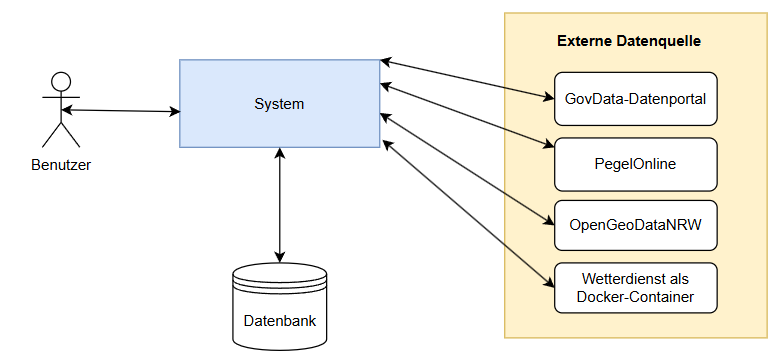
\includegraphics[width=12cm]{Kontextangrenzung.png}
	\caption{\label{} Kontextangrenzung}
\end{figure}
\section*{\large \textbf{Bausteinschicht}}
Die Bausteinschicht zeigt den näheren Aufbau des Systems - und zwar denjenigen Teil, den entwickelt wird. Jedes mit blau gefüllte Package beinhaltet alle Entitäten und die für den Aufbau der View und Datenaustausch mit der externen Datenquelle benötigten Komponenten.\\
Im Package \textbf{MainView} wird die Anwendung mit Startseite initialisiert und die Anbindung der weitern Views an die Hauptview ermöglicht. Das Package \textbf{Utils} beinhaltet zahlreiche Hilfsfunktionen. Diese dienen vor allem dazu, die Modularität, die Wartbarkeit und die Verständlichkeit des Codes sicherzustellen. Das Package \textbf{Konfiguration} beinhaltet unterschiedliche Konfigurationsklassen für die Applikation.\\ Die anderen Packages sind gemäß dem Single Responsibility Principle (SRP) aufgebaut. Jedes Package verfolgt dabei eine klar definierte, spezifische Aufgabe. Durch die Anwendung des SRP werden die Verantwortlichkeiten innerhalb des Systems präzise getrennt, was die Projektstruktur übersichtlicher und verständlicher macht.
\begin{figure}[H]
	\centering
	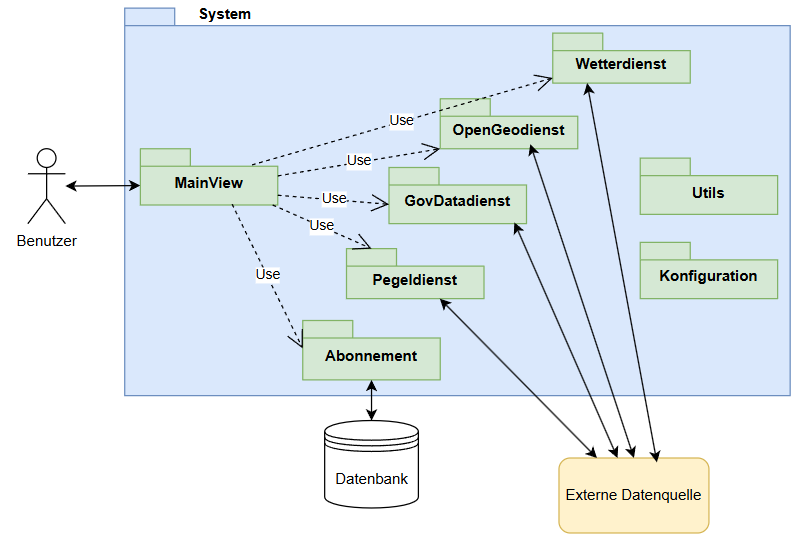
\includegraphics[width=15cm]{Bausteinsicht-1.png}
	\caption{\label{} Bausteinsicht}
\end{figure}


\section{Design-Entscheidung}
	
	
\chapter{Implementierung}
In diesem Kapitel wird über die Implementierung einzelner wichtiger Komponenten für die zuvor gewählte Architektur berichtet und ebenfalls auf während der Umsetzung auftretende Schwierigkeiten eingegangen. 
\section{Übersicht über wichtige Klassen und Entitäten}
Wie bereits am Anfang des 2.Kapitels erwähnt, wird als Einstiegspunkt für die Entwicklung eine Vaadin Applikation durch Bereitstellung von Vaadin Initializer genommen. Dies Package enthält die grundlegenden Komponente für eine simple Benutzeroberfläche. 
	
In diesem Package gibt es eine kurz Main-Klasse(\textbf{Application.java}) als Startpunkt für die Applikation, die folgenden Aufbau hat: \\
\begin{lstlisting}
@SpringBootApplication
@Theme(value = "opendata-konnektor")
@EnableCaching
public class Application implements AppShellConfigurator {
	public static void main(String[] args) {
		SpringApplication.run(Application.class, args);
	}
}
\end{lstlisting}
	Die Annotation \textbf{@SpringBootApplication} kombiniert aus:
		\begin{enumerate}
			\item  \textbf{@Configuration}: markiert die Klasse als Konfigurationsklasse für Spring.
			\item  \textbf{@EnableAutoConfiguration}: ermöglicht die automatische Konfiguration basierend auf den Abhängigkeiten im Klassenpfad.
			\item  \textbf{@ComponentScan}: sucht nach Komponenten, Konfigurationsklassen und Services im aktuellen Pakte und allen Unterpakten.
		\end{enumerate}
	Die Annotation \textbf{@Theme(value = opendata-konnektor)} legt das Vaadin-Theme fest. \textbf{value} definiert den Namen des Themes und Themens werden verwendet, um das Erscheinungsbild der Anwendung anzupassen.\\
	Die Annotation \textbf{@EnableCaching} aktiviert die Spring Caching-Funktionalität und ermöglicht die Verwendung von Cache-Mechanismen(\textbf{@Cacheable},\textbf{@Cacheable},\textbf{@CacheEvict}).\\
	\textbf{AppShellConfigurator} ist eine Schnittstelle (\textbf{interface}) aus dem Vaadin Framework. Sie wird verwende, um die \textbf{App Shell} einer Vaadin-Anwendung zu konfigurieren. Was ist die App Shell in Vaadin ?
	\begin{itemize}
		\item Die App Shell is ein grundlegendes HTML-Dokument, das vom Server an den Client gesendet wird.
		\item Es enthält die wesentlichen Informationen wie Meta-Tags, Icons, Stylesheets usw., die bei der ersten Anfrage geladen werden.
		\item Die App Shell bleibt auch unverändert, während der Inhalt dynamisch aktualisiert wird.
	\end{itemize}
	
	Um jedes Object oder jede Entität möglichst spezifisch zu halten, wird am Anfang eine grundlegende, nicht abgeleitete Basisentität, die als Vorlage oder Basis dient, auf der andere Entitäten aufgebaut werden können, indem sie deren Eigenschaften erben, ohne diese erneut zu definieren.In Java-Programmiersprache wird dieses Verhalten als \textbf{Vererbung} bezeichnet. Als Beispiel wird die Klasse \textbf{„BaseEntity“}  erläutert:
\begin{lstlisting}
@MappedSuperclass
@Getter
@Setter
public class BaseEntity implements Comparable<BaseEntity> {
	@Id
	@GeneratedValue(generator = "generateIfNotAssigned")
	@GenericGenerator(name = "generateIfNotAssigned", strategy = "org.hibernate.id.UUIDHexGenerator")
	@Column(length = 32)
	@Access(jakarta.persistence.AccessType.PROPERTY)
	private String id;
			
	@Length(min = 1)
	@NotNull
	private String label;
			
	@Column(columnDefinition = "TEXT")
	private String description;
			
	@Column(name = "base_url")
	private String url;
			
	@Column(name = "last_updated")
	private LocalDate lastUpdated;
			
	public int compareTo(BaseEntity o) {
		return (id != null) ? id.compareTo(o.getId()) : hashCode() - o.hashCode();
	}
	@Override
	public int hashCode() {
		return (id != null) ? id.hashCode() : 1;
	}
	@Override
	public boolean equals(Object obj) {
		if (!(obj instanceof BaseEntity)) {
			return false;
		}
		BaseEntity be = (BaseEntity) obj;
		return (id != null) ? id.equals(be.getId()) : this == be;
	}
}	
\end{lstlisting}
	Die Annotation \textbf{@MappedSuperclass} kennzeichnet die Klasse als Basisklasse für andere JPA-Entitäten. Die Felder und Methoden dieser Klasse werden nicht direkt in der Datenbank abgebildet, sondern in die Tabellen der abgeleiteten Klassen integriert.Außerdem wird es verwendet, um gemeinsame Eigenschaften (\textbf{id, label}), etc. zentral zu definieren.\\ \\
	Die Annotation \textbf{@Getter} und \textbf{@Setter} sind Lombok Annotation, die automatisch Getter/Setter-Methoden für alle Felder der Klasse generiert.\\
	Die Annotation \textbf{@Id} ist ein JPA-Annotation und kennzeichnet das Primärschlüsselfeld der Entität.\\ \\
	Die Annotation \textbf{@GeneratedValue(generator = "generateIfNotAssigned")} ist ebenfalls ein JPA-Annotation und gibt an, dass der Wert für \textbf{id} automatisch generiert wird. Die Option \textbf{generator} verweist auf einen benutzerdefinierten Generator.\\ \\
	Die Annotation \textbf{@GenericGenerator)} ist eine Hibernate-spezifische Annotation und definiert einen benutzerdefinierten ID-Generator. Die Option \textbf{name} ist der Name des Generators, hier „generateIfNotAssigned". Die Option \textbf{strategy} ist die Strategie für die ID-Erzeugung, und \textbf{UUIDHexGenerator} generiert UUIDs als Hex-Strings(32 Zeichen).\\ \\
	Die Annotation \textbf{@Access(jakarta.persistence.AccessType.PROPERTY)} definiert, wie auf Felder/Methoden zugegriffen wird. In diesem Fall erfolgt der Zugriff mit \textbf{PROPERTY} über Getter und Setter-Methoden. \\ \\
	Die Annotation \textbf{@Length(min = 1)} ist eine Hibernate-Validator Annotation und legt die minimale Länge für das Feld auf 1 Zeichen fest.\\
	Die Annotation \textbf{@NotNull} ist ein Bean Validation Annotation und verhinder, dass \textbf{label} auf \textbf{null} gesetzt wird und immer einen Wert haben muss.\\
	Die Annotation \textbf{@Column(columnDefinition = "TEXT")} ist JPA Annotation und definiert die Datenbankspalte \textbf{description} als \textbf{TEXT} und \textbf{TEXT} erlaubt lange Zeichenketten (mehr als \textbf{VARACHAR}). 
\begin{lstlisting}
	implements Comparable<BaseEntity>
\end{lstlisting} Damit kann die Klasse verglichen und sortiert werden, basierend auf der \textbf{id}  in der Methode \textbf{compareTo}.
	Die Annotation \textbf{@Override} stellt sicher, dass die Methode die korrekte Signatur aus dem \textbf{Comparable} Interface hat. \\ \\
	Um die Verwendung der obigen beschriebenen Klasse zu veranschaulichen, wird als Beispiel die Klasse \textbf{„Abonnement“}  erläutert:
\begin{lstlisting}
@Entity
@Table(name = "abonnement")
@Getter
@Setter
@NoArgsConstructor
@AllArgsConstructor
public class Abonnement extends BaseEntity {
	@Column(name = "file_format")
	private String dateiFormat;
	private String parameter;
	@Column(name = "location_id")
	private String locationId;
	@Column(name = "start_datum")
	private LocalDate startDatum;
	@Column(name = "end_datum")
	private LocalDate endDatum;
	@Column(name = "sub_url")
	private String subscriptionUrl;
}
\end{lstlisting}
	Die Klasse \textbf{Abonnement} erbt von der Basisklasse \textbf{BaseEntity}. Dadurch übernimmt sie automatisch alle Eigenschaften (\textbf{id,label,description,url,etc.}) und Methoden(\textbf{compareTo, hashCode, equals}) der Basisklasse.\\
	Die Annotation \textbf{@Enity} markiert die Klasse als JPA-Entität und wird in der Datenbank als Tabelle gespeichert. Die Annotation \textbf{@NoArgsConstructor} (Lombok) generiert einen parameterlosen Konstruktor und \textbf{@AllArgsConstructor} hingegen einen Konstruktor mit allen Feldern als Parameter.\\ \\
	Anschließend an die Entität, wird das zugehörige Repository, in Form eines Interfaces implementiert. Es erweitert \textbf{JpaRepository}, wodurch eine Vielzahl von CRUD-Operationen und zusätzlichen Methoden bereitgestellt werden.
\begin{lstlisting}
@Repository
public interface AbonnementRepository extends JpaRepository<Abonnement, String>{}
\end{lstlisting}
	Die Annotation \textbf{@Repository} kennzeichnet die Schnittstelle als Datenbank-Repository und wird von Spring verwendet, um die Klasse als Datenzugriffsschicht zu erkennen und ermöglicht die automatische Fehlerbehandlung bei Datenbankoperationen.\\
	\textbf{JpaRepository$<$T, ID$>$} ist eine generische Schnittstelle, die CRUD-Methoden bereitstellt:
	\begin{itemize}
		\item T : die Entitätsklasse, die verwaltet wird, in diesem Fall(Abonnement).
		\item Id: der Datentyp des Primärschlüssels (String).
	\end{itemize}
	\vspace{1cm}
	Für die Entität \textbf{Abonnement} wird ein sogenannten AbonnementController bereitgestellt, mit dem der Zugriff auf die Daten von außen ermöglicht.
\begin{lstlisting}
@RestController
@RequestMapping("/api/subscription")
public class AbonnementController {
	
	@Autowired
	private AbonnementService abonnementService;
			
	@GetMapping(value = "/data")
	public ResponseEntity<String> getAboData(@RequestParam @NotBlank String id) {
		return abonnementService.fetchAbonnementData(id).orElseGet(() -> ResponseEntity.status(HttpStatus.NOT_FOUND).body("kein Abonnement fuer die " + id + "gefunden.))
	}
			
	@GetMapping(value = "/incremental_data")
	public ResponseEntity<String> getIncrementalData(@RequestParam @NotBlank String id) {
		return abonnementService.fetchInrementalData(id).orElseGet(
		() -> ResponseEntity.status(HttpStatus.NOT_FOUND).body("Kein Abonnement fuer die " + id + " gefunden."));
	}
}
\end{lstlisting}
Die Annotation \textbf{@RestController} ist eine Kombination aus \textbf{@Controller} und \textbf{@ResponseBody} und markiert diese Klasse als REST-Controlle und die Methodenrückgaben werden automatisch in HTTP-Responses konvertiert.\\ \\
Die Annotation \textbf{@RequestMapping(/api/subscription)} definiert den Basis-URL-Pfad für alle Endpunkte in dieser Klasse.
Mit der Annotation \textbf{@Autowired} sucht Spring automatisch nach einer passenden Bean und injiziert diese in das Controller-Feld \textbf{abonnementService}. Dies ist in Spring als \textbf{Dependency Injection} genannt.\\ \\
Die Annotation \textbf{@GetMapping(/data)} definiert einen GET-Endpunkt unter /api/subscription/data und \textbf{@RequestParam} extrahiert den \textbf{id}-Parameter aus der URL-Abfragezeichenkette. \textbf{@NotBlank} ist ein Bean Validation und validiert, dass der \textbf{id}-Parameter nicht leer ist und falls der leer ist, wird ein 400 Bad Request zurückgegeben. \textbf{ResponseEntity$<$String$>$} wird verwendet, um eine HTTP-Response mit einem StatusCode und einem Body zurückzugeben.
	
\section{Front-End-Komponente }
Im Rahmen dieses Abschnittes wird die Implementierung des Use-Cases \textit{Datenstream eines Klimaphänomen einsehen} erläutert. Die Entwicklung erfolgt unter Verwendung von Vaadin-Framework.\\ \\
Die Umsetzung eines UI-Komponents erfolgt unter Java-Programmiersprache als Klasse, welche ein Komponent wie z.B. ein VerticalLayout oder HorizontalLayout oder ein Dialog von Paket \textbf{com.vaadin.flow.component.Component} erbt.
\begin{lstlisting}
import com.vaadin.flow.component.combobox.ComboBox;
import com.vaa
din.flow.component.orderedlayout.HorizontalLayout;
import com.vaadin.flow.component.orderedlayout.VerticalLayout;
		
@Route(value = "suche", layout = MainLayout.class)
@Slf4j
public class SearchGeoDataView extends VerticalLayout {
			
	private ComboBox<String> tfSearch = new ComboBox<>();
	tfSearch.setPlaceholder("Suche nach Phaenomen");
	tfSearch.setClearButtonVisible(true);
	List<String> phaenomenList = List.of("Niederschlag", "Grundwasser", "Pegel", "Bodentemperatur",
	"Lufttemperatur", "Luftfeuchtigkeit", "Windgeschwindigkeit", "Windrichtung", "Windstärke", "Windböe",
	"Sonnenscheindauer", "Gesamtbewölkung");
	tfSearch.setItems(phaenomenList.stream().sorted().toList());
	tfSearch.setAllowCustomValue(true);
	tfSearch.setWidth("20%");
	tfSearch.getStyle().set("borderRadius", "12px").set("padding", "0.5rem 1rem")
	.set("boxShadow", "0 2px 6px rgba(0, 0, 0, 0.1)").set("backgroundColor", "#fff");
		
	HorizontalLayout searchLayout = new HorizontalLayout(tfSearch);
	searchLayout.setWidthFull();
	searchLayout.setJustifyContentMode(JustifyContentMode.CENTER);
	add(searchLayout);
}
\end{lstlisting}
Mit dem obigen Code ergibt sich folgende Abbildung ohne die Navigationsleiste: 
\begin{figure}[h!]
	\centering
	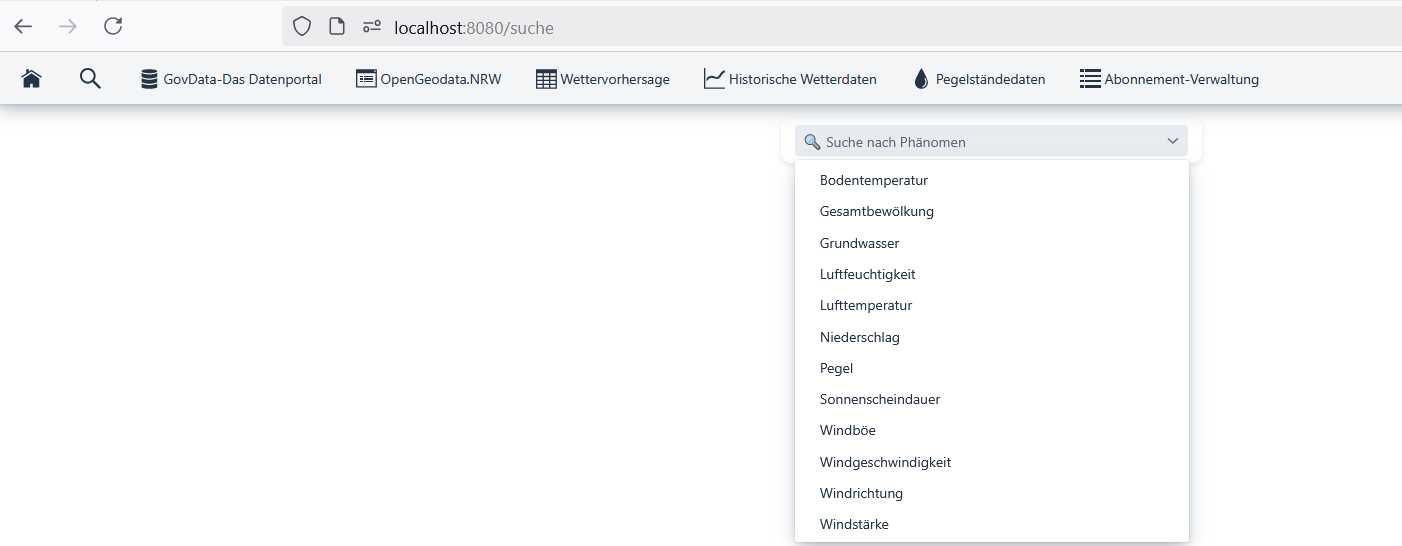
\includegraphics[width=17cm]{suchSeite.png}
	\caption{\label{suche:Seite}Suche Seite}
\end{figure}
	
Wie üblich in Java, initialisiert man ein Komponente in Vaadin auch mit dem Schlüsselwort \textbf{new}. Bei dem Beispiel wird ein DropDown-Feld zur Auswahl von \textbf{String}-Werten erstellt.\\ \\
Mit Abruf von \textbf{tfSearch.getStyle()} wird dies Dropdown stilisiert und mit \textbf{tfSearch.setItems(...)} mit vordefinierten Phänomenen gefüllt. Mit \textbf{HorizontalLayout searchLayout = new HorizontalLayout(tfSearch)} wird ComboBox in ein \textbf{HorizontalLayout}  eingebettet und zentriert ausgerichtet.\\
Am Ende mit \textbf{add(searchLayout)} wird das Layout zur Benutzeroberfläche hinzugefügt.\\ \\
Zurück zu der Navigationsleiste, um so einen Leiste in Vaadin erstellen zu können, wird anhand des Code ins Details eingegangen.\\

Die Annotation \textbf{@Layout} wird verwendet, um die Klasse als Layout festzulegen. In Vaadin bestimmt ein Layout, wie der Seiteninhalt strukturiert wird, insbesondere wie Komponenten innerhalb des Layouts angeordnet werden.\\	

Die Annotation \textbf{@AnonymousAllowed} erlaubt es anonymen Benutzern (nicht authentifizierten Benutzern), auf dieses Layout zuzugreifen. Ohne diese Annotation wäre der Zugriff auf diese Klasse möglicherweise eingeschränkt.
\begin{lstlisting}
@Layout
@AnonymousAllowed
public class MainLayout extends AppLayout {
	public MainLayout() {
		addToNavbar(createHeaderContent());
	}
	private Component createHeaderContent() {
		Header header = new Header();
		header.addClassNames(BoxSizing.CONTENT, Display.FLEX, FlexDirection.COLUMN, Width.FULL);
				
		Nav navMain = new Nav();
		navMain.addClassNames(Display.FLEX, Overflow.AUTO, Padding.Horizontal.MEDIUM, Padding.Vertical.XSMALL,
		TextColor.PRIMARY, BoxShadow.MEDIUM, Width.FULL);
		UnorderedList navMainItemList = new UnorderedList();
		navMainItemList.addClassNames(Display.INLINE_FLEX, Gap.LARGE, ListStyleType.NONE, Margin.NONE, Padding.SMALL,
		TextColor.PRIMARY);
		navMain.add(navMainItemList);
				
		for (MenuItemInfo menuItem : createMainMenuItems()) {
			navMainItemList.add(menuItem);
		}
				
		HorizontalLayout navControls = new HorizontalLayout();
		navControls.setSpacing(false);
		navControls.setJustifyContentMode(FlexComponent.JustifyContentMode.BETWEEN);
		navControls.add(navMain);
		header.add(navControls);
		return header;
	}
			
	private MenuItemInfo[] createMainMenuItems() {
		return new MenuItemInfo[] { new MenuItemInfo(null, VaadinIcon.HOME.create(), StartView.class),
			new MenuItemInfo(null, VaadinIcon.SEARCH.create(), SearchGeoDataView.class),
			new MenuItemInfo("GovData-Das Datenportal", VaadinIcon.DATABASE.create(), GridGovData.class),
			new MenuItemInfo("OpenGeodata.NRW", VaadinIcon.MODAL_LIST.create(), OpenDataNrwView.class),
			new MenuItemInfo("Wettervorhersage", VaadinIcon.TABLE.create(), WettervorhersageView.class),
			new MenuItemInfo("Historische Wetterdaten", VaadinIcon.SPLINE_CHART.create(),
			HistoricalWetterDatenView.class),
			new MenuItemInfo("Pegelständedaten", VaadinIcon.DROP.create(), PegelstandView.class),
			new MenuItemInfo("Abonnement-Verwaltung", VaadinIcon.LINES_LIST.create(), GridAbonnement.class) };
	}
			
	public static class MenuItemInfo extends ListItem {
		private final Class<? extends Component> view;
		public MenuItemInfo(String menuTitle, Component icon, Class<? extends Component> view) {
			this.view = view;
			RouterLink link = new RouterLink();
			link.addClassNames(Display.FLEX, Gap.XSMALL, Height.MEDIUM, AlignItems.CENTER, Padding.Horizontal.SMALL,
			TextColor.BODY);
			link.setRoute(view);
			Span text = new Span(menuTitle);
			text.addClassNames(FontWeight.MEDIUM, FontSize.MEDIUM, Whitespace.NOWRAP);
					
			if (icon != null) {
				link.add(icon);
			}
			link.add(text);
			add(link);
		}
		public Class<?> getView() {
			return view;
		}
	}
}
\end{lstlisting}
Die Klasse \textbf{MainLayout} erweitert \textbf{AppLayout},welches in Vaadin ein standardisiertes Layout ist, das eine Navigationsleiste und einen Inhaltsbereich definiert. Im Konstruktor wird \textbf{createHeaderContent()} aufgerufen und zum Navigationsbereich (\textbf{Navbar}) hinzufügt.\\ 

Die Methode \textbf{createHeaderContent()} erstellt den Header-Bereich der Anwendung. Die Komponente \textbf{Header} wird erstellt und gestylt. Das Navigationselement mit \textbf{Nav} wird erstellt und eine \textbf{UnorderedList} wird hinzugefügt. Für jedes \textbf{MenuItemInfo} wird ein Listenelement \textbf{ListItem} hinzufügt. Der Header wird zurückgegeben und in die Navbar eingefügt.\\

Die Methode \textbf{createMainMenuItems()} erzeugt ein Array von \textbf{MenuItemInfo}- Objekten. Jedes \textbf{MenuItemInfo}- Objekte repräsentiert einen Menüpunkt mit einem Titel, einem Icon und einer zugehörigen View-Klasse. \\

Die innere Klasse \textbf{MenuItemInfo} erweitert \textbf{ListItem} und stellt ein Navigationsmenüelement dar. Konstruktor erstellt einen \textbf{RouterLink}, fügt optional Icon und den Text hinzu. Die Methode \textbf{getView()} gibt die View-Klasse zurück, die beim Klicken auf das Menüelement aufgerufen wird.
\clearpage
Wählt man nun einen Eintrag aus der DropDownList aus,z.B.\textbf{Pegel}, ergibt sich folgende Abbildung:
\begin{figure}[H]
	 \centering
	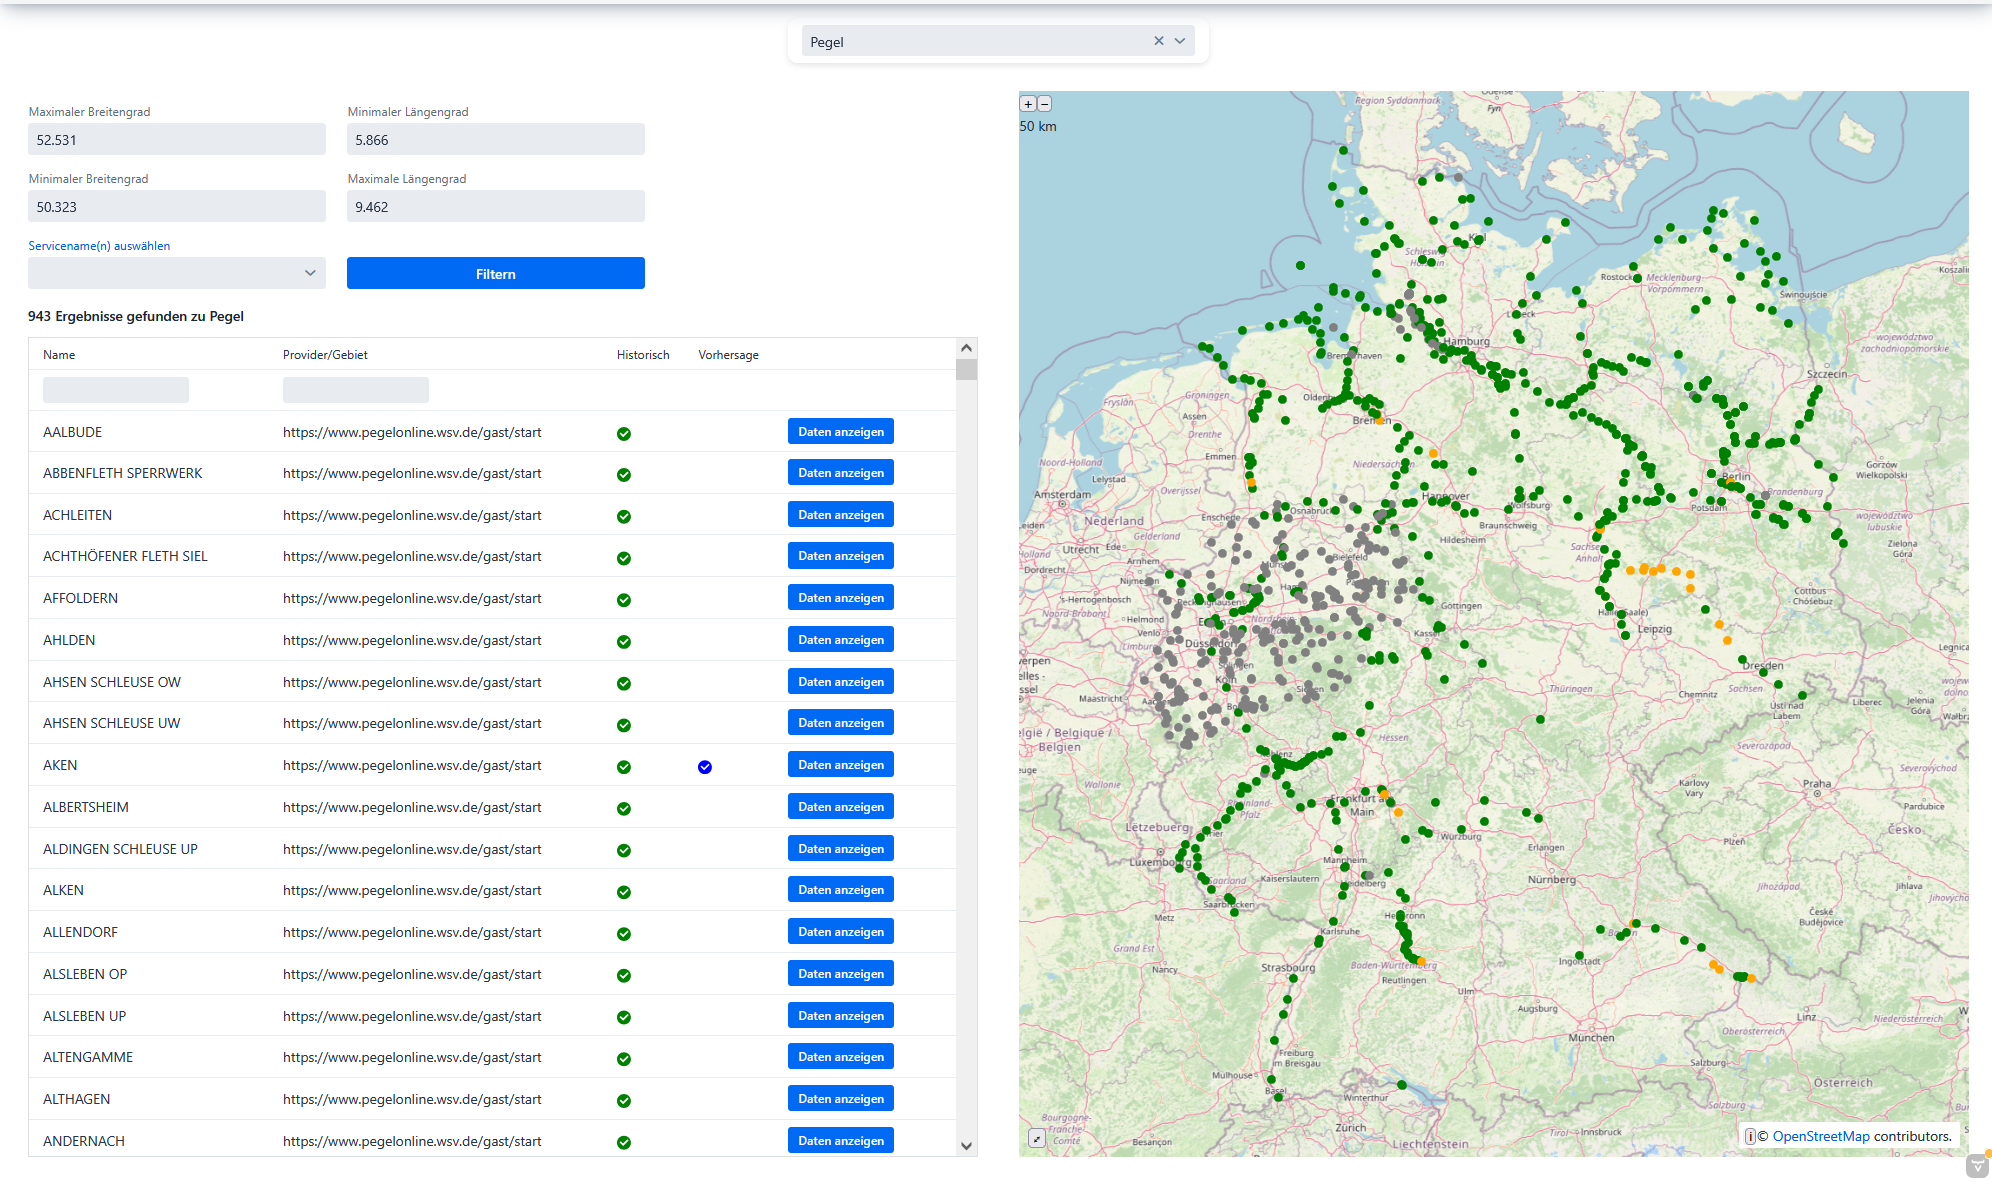
\includegraphics[width=18cm]{pegel.png}
	\caption{\label{pegel:}Pegel}
\end{figure}
Bei der Abbildung sind es drei Hauptkomponenten deutlich zu erkennen, nämlich : die Tabelle, die Karte und die Filtermöglichkeiten nach Koordinaten und Servicename.
\section*{\small \textbf{1. Die Tabelle}}
In Vaadin wird eine Tabelle als Grid genannt und wird in dem Code wie folgt initialisiert.
\begin{lstlisting}
private Grid<StationDTO> stationGrid = null;

private Grid.Column<StationDTO> nameColumn = null;
private Grid.Column<StationDTO> providerColumn = null;
private Grid.Column<StationDTO> historischColumn = null;
private Grid.Column<StationDTO> vorhersageColumn = null;
private Grid.Column<StationDTO> btnColumn = null;
private StationDTOFilter filter;
private HeaderRow headerRow = null;
private StationDTO currentStation = null;

private void initGridStation() {
	stationGrid = new Grid<>(StationDTO.class, false);
	dataProviderStations = stationGrid.setItems(mergedStations);
	
	nameColumn = stationGrid.addColumn(station -> station.getName()).setHeader("Name")
	.setAutoWidth(true).setFlexGrow(1);
	providerColumn = stationGrid.addColumn(station -> station.getProvider()).setHeader("Provider/Gebiet")
	.setAutoWidth(true).setResizable(true).setFlexGrow(1);
	historischColumn = stationGrid.addColumn(new ComponentRenderer<>(station -> {
		if (station instanceof WetterStationDTO wetter) {
			Icon statusIndicator = new Icon();
			if (wetter.getIsHistorical() != null && wetter.getIsHistorical()) {
				statusIndicator = VaadinIcon.CHECK_CIRCLE.create();
				statusIndicator.setColor("green");
				statusIndicator.addClassName("text-body");
				statusIndicator.setSize("1em");
			}
			return statusIndicator;
		}
		if (station instanceof PegelStationDTO pegel) {
			Icon statusIndicator = new Icon();
			if (pegel.getIsHistorical() != null && pegel.getIsHistorical()) {
				statusIndicator = VaadinIcon.CHECK_CIRCLE.create();
				statusIndicator.setColor("green");
				statusIndicator.addClassName("text-body");
				statusIndicator.setSize("1em");
			}
			return statusIndicator;
		}
		return null;
	})).setHeader("Historisch").setAutoWidth(true).setFlexGrow(0);
	
	vorhersageColumn = stationGrid.addColumn(new ComponentRenderer<>(station -> {
		if (station instanceof WetterStationDTO wetter) {
			Icon statusIndicator = new Icon();
			if (wetter.getIsForecast() != null && wetter.getIsForecast()) {
				statusIndicator = VaadinIcon.CHECK_CIRCLE.create();
				statusIndicator.setColor("blue");
				statusIndicator.addClassName("text-body");
				statusIndicator.setSize("1em");
			}
			return statusIndicator;
		}
		if (station instanceof PegelStationDTO pegel) {
			Icon statusIndicator = new Icon();
			if (pegel.getIsForecast() != null && pegel.getIsForecast()) {
				statusIndicator = VaadinIcon.CHECK_CIRCLE.create();
				statusIndicator.setColor("blue");
				statusIndicator.addClassName("text-body");
				statusIndicator.setSize("1em");
			}
			return statusIndicator;
		}
		return null;
	})).setHeader("Vorhersage").setAutoWidth(true).setFlexGrow(0);
	
btnColumn = stationGrid.addColumn(new ComponentRenderer<>(st -> {
	Button btnShowData = new Button("Daten anzeigen");
	btnShowData.addThemeVariants(ButtonVariant.LUMO_SMALL, ButtonVariant.LUMO_PRIMARY);
		
	btnShowData.addClickListener(click -> {
	if (dialogData == null) {
		dialogData = new Dialog();
	} else {
		dialogData.removeAll();
		dialogData = new Dialog();
	}
	....
	// Weitere Logik fuer die Datenverarbeitung
	});
	return btnShowData;
})).setAutoWidth(true).setFlexGrow(1);
	
stationGrid.setColumnOrder(nameColumn, providerColumn, historischColumn, vorhersageColumn, btnColumn);
stationGrid.setSizeFull();
	
stationGrid.getHeaderRows().clear();
headerRow = stationGrid.appendHeaderRow();
filter = new StationDTOFilter(dataProviderStations);
headerRow.getCell(nameColumn).setComponent(createFilterHeader(filter::setStationName));
headerRow.getCell(providerColumn).setComponent(createFilterHeader(filter::setProvider));
\end{lstlisting}

Bei dem Code-Abschnitt wird ein \textbf{Grid<StationDTO>} initialisiert und es erstellt fünf Spalten:
\begin{enumerate}
\item \textbf{Name} – Zeigt den Namen der Station an.
\item \textbf{Provider/Gebiet} – Zeigt den Anbieter oder das Gebiet der Station an.
\item \textbf{Historisch} – Zeigt ein grünes Icon an, wenn die Station historisch ist (getIsHistorical() ist true)
\item \textbf{Vorhersage} – Zeigt ein blaues Icon an, wenn Vorhersagedaten verfügbar sind (getIsForecast() ist true).
\item \textbf{Daten anzeigen} – Fügt einen Button hinzu, der beim Klicken ein Dialogfenster zur Datenanzeige öffnet.
\item Zusätzlich wird ein HeaderRow für die Filterung hinzugefügt, der Filter für Name und Provider ermöglicht.
\end{enumerate}


\section*{\small \textbf{2. Die Karte}}
Die Karte ist eine Komponente, die an vielen Stellen in der Applikation wiederverwendbar ist, deswegen ist es sinnvoll, diese als eine eigene Klasse auszulagern.\\
Die Methode zum Aufruf der Karte-Komponente:
\begin{lstlisting}
private void initOpenLayersMap() {
  if (!mapVerticalLayout.getChildren().anyMatch(component -> component instanceof OpenLayersMap)) {
	olMap = new OpenLayersMap();
	olMap.setSizeFull();
	olMap.showStationsOnMap(dataProviderStations.getItems().collect(Collectors.toList()));
    mapVerticalLayout.add(olMap);
  } else {
	olMap.showStationsOnMap(dataProviderStations.getItems().collect(Collectors.toList()));
  }
}
\end{lstlisting}
Die Methode \textbf{initOpenLayersMap()} initialisiert eine \textbf{OpenLayersMap}-Komponente in einem Vaadin-Layout :
\begin{itemize}
\item prüft, ob bereits eine \textbf{OpenLayersMap} im \textbf{mapVerticalLayout} vorhanden ist.
\item Falls nicht vorhanden, wird eine neue  \textbf{OpenLayersMap} erstellt und den Stationen aus dem  \textbf{dataProviderStations}-Datensatz hinzugefügt.
\item Falls bereits vorhanden, wird die bestehende Karte aktualisiert, um die Stationen anzuzeigen.
\item Ein \textbf{DataProvider} in Vaadin ist eine Datenquelle, die Daten für UI-Komponenten wie Grids bereitstellt. Es verwaltet die Daten und stellt Methoden zur Verfügung, um Daten zu filtern, zu sortieren und zu aktualisieren.
\end{itemize}

\begin{lstlisting}
@NpmPackage(value = "ol", version = "8.2.0")
@NpmPackage(value = "ol-ext", version = "4.0.13")
@NpmPackage(value = "ol-layerswitcher", version = "4.1.1")
@NpmPackage(value = "ol-popup", version = "5.1.0")
@Tag("openlayers")
@JsModule("./src/openlayers-connector.js")
@Slf4j
public class OpenLayersMap extends Div {
	public OpenLayersMap() {
		this.getParent().ifPresent(null);
		initConnector();
		
		addDetachListener(detach -> {
			shutDown();
		});
	}
	public <T extends RestDTO> void showStationsOnMap(List<T> stations) {
		runBeforeClientResponse(ui -> {
			boolean isWetterstation = false;
			if (stations != null && !stations.isEmpty()) {
				isWetterstation = stations.get(0) instanceof WetterStationDTO;
			}
			String jsArray = buildStationsJson(stations);
			ui.getPage()
			.executeJs("window.Vaadin.Flow.openLayersConnector.showStations($0, $1, $2)", getElement(),
			jsArray, isWetterstation);
		});
	}
	private <T extends RestDTO> String buildStationsJson(List<T> stations) {
		try {
			if (stations == null || stations.isEmpty()) {
				return "[]";
			}
			return objectMapper.writeValueAsString(stations);
		} catch (Exception e) {
			e.printStackTrace();
			return "[]";
		}
	}
	private void initConnector() {
		runBeforeClientResponse(ui -> ui.getPage()
		.executeJs("window.Vaadin.Flow.openLayersConnector.initLazy($0)", getElement()));
	}
}
\end{lstlisting}

Die Klasse \textbf{OpenLayersMap} erweitert Div und integriert eine  \textbf{OpenLayers}-Kartenkomponente.\\
Annotationen:
\begin{itemize}
\item \textbf{@NpmPackage}: importiert JavaScript-Pakete (ol, ol-ext, ol-layerswitcher, ol-popup) in der angegebenen Version.
\item \textbf{@Tag}: definiert das HTML-Tag als \textbf{openlayers}.
\item \textbf{@JsModule}: verweist auf die JavaScript-Datei \textbf{openlayers-connector.js} zur Client-Integration.
\end{itemize}
Methoden:
\begin{itemize}
	\item \textbf{showStationsOnMap(List<T> stations)}: zeigt Stationen auf der Karte an und erkennt, ob es sich um Wetterstationen handelt.
	\item \textbf{buildStationsJson(List<T> stations)}: konvertiert die Stationen-Liste in ein JSON-Array für die Client-Seite.
	\item \textbf{initConnector()}: Initialisiert den JavaScript-Connector(initLazy).
\end{itemize}

\section*{\small \textbf{3. Die Filtermöglichkeiten}}
\begin{lstlisting}
private FormLayout formLayout = new FormLayout();
private TextField tfMinLatitude = new TextField("Minimaler Breitengrad");
private TextField tfMaxLatitude = new TextField("Maximaler Breitengrad");
private TextField tfMinLongitude = new TextField("Minimaler Längengrad");
private TextField tfMaxLongitude = new TextField("Maximale Längengrad");
private Button btnFilterStations = new Button("Filtern");

tfMinLatitude.setPlaceholder("Minimaler Breitengrad eingeben (47.2701 bis 55.0581)");
tfMaxLatitude.setPlaceholder("Maximaler Breitengrad eingeben (47.2701 bis 55.0581)");
tfMinLongitude.setPlaceholder("Minimaler Längengrad eingeben  (5.8663 bis 15.0419)");
tfMaxLongitude.setPlaceholder("Maximaler Längegrad eingeben (5.8663 bis 15.0419)");
tfMinLatitude.setValue("50.323");
tfMaxLatitude.setValue("52.531");
tfMinLongitude.setValue("5.866");
tfMaxLongitude.setValue("9.462");

btnFilterStations.addThemeVariants(ButtonVariant.LUMO_PRIMARY);
btnFilterStations.addClickListener(submit -> {
	double minLat = Double.parseDouble(tfMinLatitude.getValue());
	double maxLat = Double.parseDouble(tfMaxLatitude.getValue());
	double minLon = Double.parseDouble(tfMinLongitude.getValue());
	double maxLon = Double.parseDouble(tfMaxLongitude.getValue());
	
	if (ddProvider.getValue() != null) {
		ddProvider.setValue(null);
	}
	
	List<StationDTO> filteredStations = mergedStations.stream()
	.filter(station -> station.getLatitude() >= minLat && station.getLatitude() <= maxLat
	&& station.getLongitude() >= minLon && station.getLongitude() <= maxLon)
	.collect(Collectors.toList());
	
	if (filteredStations.isEmpty()) {
		Utils.showHinweisBox("Keine Stationen innerhalb der Bounding Box gefunden.");
	} else {
		dataProviderStations = stationGrid.setItems(filteredStations);
		initOpenLayersMap();
		updateHeaderRows();
	}
	countResult.setText(dataProviderStations.getItemCount() + " Ergebnisse gefunden zu " + tfSearch.getValue());
});
formLayout.setWidth("65%");
formLayout.setResponsiveSteps(new FormLayout.ResponsiveStep("0", 1), 
new FormLayout.ResponsiveStep("500px", 2));
\end{lstlisting}
Dieser Code-Abschnitt erstellt ein Formular zur Filterung von Stationen anhand von Koordinaten (Breitengrad und Längengrad).\\
Formularkomponenten:
\begin{itemize}
	\item \textbf{Vier Textfelder:}: Eingabe von minimalen und maximalen Breiten- und Längengraden.
	\item Button \textbf{Filtern}: Startet den Filterprozess.
\end{itemize}
Filterlogik beim Button-Klick:
\begin{itemize}
	\item holt die eingegebenen Koordinaten und filtert die mergedStations-Liste.
	\item aktualisiert \textbf{dataProviderStations} mit den gefilterten Stationen.
	\item aktualisiert die Karte mit \textbf{initOpenLayersMap()} und die Header-Row.
\end{itemize}

\begin{lstlisting}
private Map<String, List<? extends StationDTO>> providerList = new HashMap<>();
ddProvider.setLabel("Servicename(n) auswählen");
ddProvider.setItemLabelGenerator(String::toString);
ddProvider.setWidth("20%");
	
ddProvider.addValueChangeListener(event -> {
	stationGrid.getHeaderRows().clear();
	if (event.getValue() != null) {
		List<? extends StationDTO> selectedStations = providerList.get(event.getValue());
		if (selectedStations != null) {
		if (tfMaxLatitude.getValue() != null && tfMinLongitude.getValue() != null) {
			GridListDataView<StationDTO> dataView = stationGrid.getListDataView();
			if (event.getValue().equals("OpenGeoData-NRW")) {
					dataView.setFilter(st -> selectedStations.contains(st));
					providerColumn.setHeader("Gebiet");
			} else if (event.getValue().equals("Pegelonline-Dienst")) {
					dataView.setFilter(st -> selectedStations.contains(st));
					providerColumn.setHeader("Provider");
			} else {
					dataView.setFilter(st -> st.getProvider().equals(event.getValue()));
					providerColumn.setHeader("Provider");
			}
			dataProviderStations = dataView;
		} else {
			if (event.getValue().equals("OpenGeoData-NRW")) {
				providerColumn.setHeader("Gebiet");
			} else {
				providerColumn.setHeader("Provider");
			}
				dataProviderStations = stationGrid.setItems(selectedStations.stream()
				.sorted(Comparator.comparing(StationDTO::getName)).collect(Collectors.toList()));
			}
			updateHeaderRows();
		} else {
			providerColumn.setHeader("Provider/Gebiet");
			dataProviderStations = stationGrid.setItems(mergedStations);
			updateHeaderRows();
		}
		stationGrid.getDataProvider().refreshAll();
		initOpenLayersMap();
		countResult.setText(dataProviderStations.getItemCount() + " Ergebnisse zu " + tfSearch.getValue()
		+ (event.getValue() != null ? " von " + event.getValue() : ""));
});
\end{lstlisting}
Dieser Code-Abschnitt implementiert die Filterlogik für den Dropdown-Provider.\\
Filterlogik bei Wertänderung:
\begin{itemize}
	\item Überprüft, ob ein Dienstanbieter \textbf{(event.getValue())} ausgewählt ist:
	\begin{itemize}
		\item falls Koordinatenfilter aktiv: verwendet \textbf{GridListDataView}, um die gefilterten Stationen weiter zu filtern.
		\item falls kein Koordinatenfilter: sortiert und setzt die Stationen basierend auf dem Dienstanbieter und aktualisiert die Header-Überschrift.
	\end{itemize}
	\item Falls kein Anbieter ausgewählt ist: setzt die ursprüngliche List als Datensatz und setzt die Standard-Header-Überschrift.
	\item Aktualisiert die Karte mit \textbf{initOpenLayersMap()} und die Header-Zeilen. 
\end{itemize}
\textbf{GridListDataView} ist eine Schnittstelle in Vaadin, die es ermöglicht, die Daten eines Grid-Components zu verwalten und zu manipulieren.
\clearpage
Wenn \textbf{OpenGeoData-NRW} als Eintrag aus dem Dropdown ausgewählt wird, ergibt sich folgende Abbildung:
\begin{figure}[H]
	\centering
	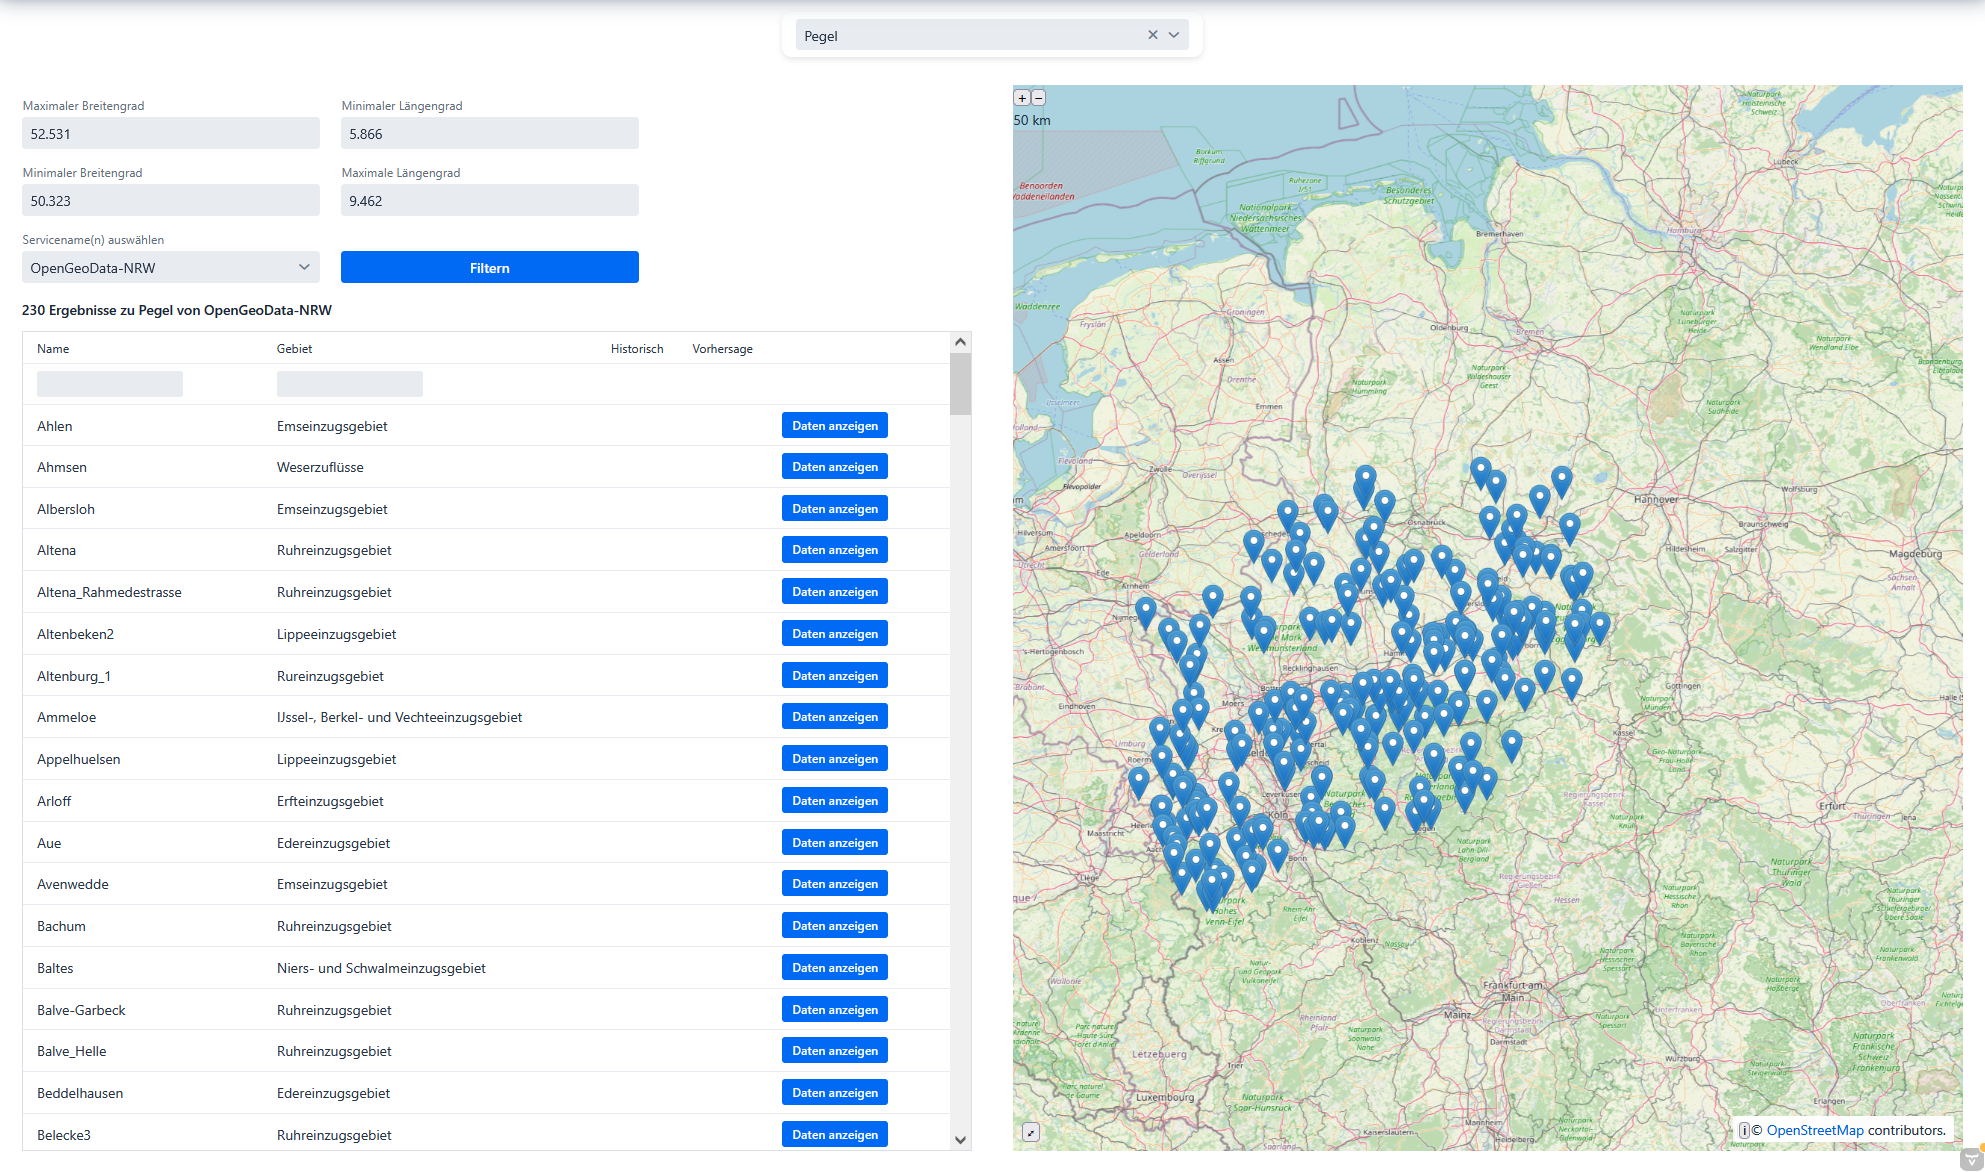
\includegraphics[width=18cm]{pegel-opengeodata.png}
	\caption{\label{pegel:}Pegel-OpenGeoDataNrw}
\end{figure}



\chapter{Evaluierung}
	
\chapter{Fazit und Ausblick}
	
\printbibliography
\end{document}